\documentclass[mathserif]{beamer}
\usepackage{beamerthemeshadow}
\usepackage{beamerthemesplit}
%\usetheme{shadow}
\usecolortheme{default}
\setbeamertemplate{footline}[frame number]
\useinnertheme[shadow=true]{rounded}
%\setbeamertemplate{footline}{\insertframenumber/\inserttotalframenumber}
%\useoutertheme{infolines}
%\setbeamertemplate{headline}{} % removes the headline that infolines inserts

%\usetheme{boxes}
%\usepackage{amsmass}
%\usepackage{amssymb,amsfonts,url}

\usepackage{algorithm}
\usepackage{algorithmic}

\usepackage{graphicx}
\graphicspath{{Problems/}}


\usepackage{tikz}
\usetikzlibrary{shadows}
\usetikzlibrary{positioning}
\usepackage{verbatim}
\usepackage{pgfplots}
\usepackage{verbatim}
\usetikzlibrary{arrows,shapes}

\definecolor{darkblue}{rgb}{0.2,0.2,0.6}
\definecolor{darkred}{rgb}{0.6,0.1,0.1}
\definecolor{darkgreen}{rgb}{0.2,0.6,0.2}

\usetikzlibrary{shadings,shadows,shapes.arrows}

\usetikzlibrary{calc} 
\makeatletter 
\@namedef{color@3}{blue!20}
\@namedef{color@1}{green!70}   
%\@namedef{color@3}{yellow!50} 
\@namedef{color@2}{orange!90}  
%\@namedef{color@5}{magenta!70} 
%\@namedef{color@6}{yellow!70}    

\newcommand{\graphitemize}[2]{%
\begin{tikzpicture}[every node/.style={align=center}, scale=0.78]  
 \draw[fill=green!5, fill opacity=0.1, green, inner sep=0.05cm, outer sep=0.05cm] (5,0) arc(0:360:5);
 % \draw[fill=white, fill opacity=0.1, white, inner sep=0.05cm, outer sep=0.05cm] (4,0) arc(0:360:4);
%  \shade[ball color=gray!10!] (0,0) coordinate(Hp) circle (.9);
  \node[shape=circle,  minimum size=1.1cm,fill=red!60,font=\Large,outer sep =.15cm,inner sep=.2cm,drop  shadow={ashadow, color=red!60!black}](ce){#1};  
   % \shade[ball color=blue!20!] (0,0) coordinate($Algorithm$) circle (1.5cm);

\foreach \gritem [count=\xi] in {#2}  {\global\let\maxgritem\xi}  
\foreach \gritem [count=\xi] in {#2}
{% 
\pgfmathtruncatemacro{\angle}{90+360/\maxgritem*\xi}
\edef\col{\@nameuse{color@\xi}}
\node[shape=circle,
     ultra thick,
     draw=white,
     fill opacity=1,
     drop  shadow={ashadow, color=blue!60},
     fill=\col,outer sep=0.25cm,        
     minimum size=2cm] (satellite-\xi) at (\angle:5cm) {\gritem };
     \draw[line width=0.25cm,-latex, \col] (ce) -- (satellite-\xi);
     }%
% \draw[violet, fill=violet!10] (4,0) arc(0:360:4);
\end{tikzpicture}  
}%



\newcommand*{\tikzarrow}[2]{%
  \tikz[
    baseline=(A.base),             % Set baseline to the baseline of node content
    font=\footnotesize\sffamily    % Set fontsize of the node content
  ]
  \node[
    single arrow,                  % Shape of the node
    single arrow head extend=2pt,  % Actual width of arrow head
    draw,                          % Draw the node shape
    inner sep=2pt,                 % Separation between node content and node shape
    top color=white,               % Shading color on top of node
    bottom color=#1,               % Shading color on bottom of node
    drop shadow                    % Draw a shadow
  ] (A) {#2};%
}


\def\arrow{
  (10.05:1.1) -- (6.05:1) arc (6.05:120:1) [rounded corners=0.5] --
  (120:0.9) [rounded corners=1] -- (130:1.1) [rounded corners=0.5] --
  (120:1.3) [sharp corners] -- (120:1.2) arc (120:5.25:1.2)
  [rounded corners=1] -- (10.05:1.1) -- (6.05:1) -- cycle
}

\tikzset{
  ashadow/.style={opacity=.25, shadow xshift=0.07, shadow yshift=-0.07},
}

\def\arrows[#1]{         
  \begin{scope}[scale=#1]
    \draw[color=darkred, drop  shadow={ashadow, color=red!60!black}] \arrow;

    \draw[color=darkgreen, bottom color=green!90!black, top color=green!60,   drop shadow={ashadow, color=green!60!black}] [rotate=120] \arrow;

    \draw[color=darkblue, right color=blue, left color=blue!60,   drop shadow={ashadow, color=blue!60!black}] [rotate=240] \arrow;

    % to hide the green shadow
    \draw[color=darkred, left color=red, right color=red!60] \arrow;
  \end{scope}
}

\tikzstyle{vertex}=[circle,fill=black!25,draw,minimum size=20pt,inner sep=0pt]
\tikzstyle{smallvertex}=[circle,fill=black!25,draw,minimum size=10pt,inner sep=0pt]
\tikzstyle{middlevertex}=[circle,fill=black!25,draw,minimum size=15pt,inner sep=0pt]
\tikzstyle{selected vertex} = [vertex, draw,fill=red!24]
\tikzstyle{blue smallvertex} = [smallvertex, draw,fill=blue]
\tikzstyle{red smallvertex} = [smallvertex, draw,fill=red]
\tikzstyle{edge} = [draw,thick,->]
\tikzstyle{undirectededge} = [draw,thick]
\tikzstyle{weight} = [font=\small]
\tikzstyle{selected edge} = [draw,line width=5pt,-,red!50]
\tikzstyle{ignored edge} = [draw,line width=5pt,-,black!20]
\tikzstyle{squarednode}=[draw, fill=blue!20, thick, minimum size=5mm]
\tikzstyle{roundnode}=[circle, draw, fill=blue!20, thick, minimum size=5mm]



%\usepackage{CJK}
%\usepackage{pinyin}

%    \begin{figure}
%        \centering
%        \includegraphics[width=0.8\textwidth]{newGeneRep.eps}
%    \end{figure}

% \begin{figure}%
%   \begin{center}%
%     \begin{minipage}{0.70\textwidth}%
%      \includegraphics[width=1.0\textwidth]{comp25000.eps}%
%     \end{minipage}%
%     \begin{minipage}{0.30\textwidth}
%      \includegraphics[width=1.0\textwidth]{comparelabel.eps}%
%     \end{minipage}%
%   \end{center}
% \end{figure}

% \begin{table}
%   {\begin{tabular}{l|rrr}\hline
%       & \multicolumn{3}{c}{Actual number of DCJ operations}\\
%       \# genes &\# genes $\times 1$&\# genes $\times 2$&\# genes  $\times 3$ \\
% \hline
%      (a)~25,000 & 0.5\% ~~&  0.9\% ~~& 1.7\%~~\\
%       (b)~10,000 & 0.8\%~~ &  1.4\% ~~& 2.7\%~~\\
%      (c)~ 1,000 & 2.7\%~~ & 4.7\%~~ & 14.7\%~~\\ \hline
%     \end{tabular}} {}%
% \end{table}

% \begin{eqnarray}
% T(n) &=&  \sum\nolimits_{i=1}^n C_i \\
%      &=&  \# PUSH + \#POP \\
%      &<& 2\times \#PUSH \\
%      &<& 2n \\
% \end{eqnarray}

% \[ 
% \begin{matrix}
% \begin{pmatrix}
% C_{11} & C_{12} \\ 
% C_{21} & C_{22} 
% \end{pmatrix}
% =
% \begin{pmatrix}
% A_{11} & A_{12} \\ 
% A_{21} & A_{22}  
% \end{pmatrix}
% 
% \begin{pmatrix}
% B_{11} & B_{12} \\ 
% B_{21} & B_{22}  
%  
% \end{pmatrix}
%     
%    \end{matrix}
% \]
% 
% 
% \begin{eqnarray}
%  C_{11} &=& (A_{11}\times B_{11}) + (A_{12} \times B_{21}) \\
% C_{12} &=& (A_{11}\times B_{12}) + (A_{12} \times B_{22}) \\
% C_{21} &=& (A_{21}\times B_{11}) + (A_{22} \times B_{21}) \\
% C_{22} &=& (A_{21}\times B_{12}) + (A_{22} \times B_{22}) 
% \end{eqnarray}
% \begin{figure}%
%      \begin{minipage}{0.32\textwidth}%
%       \includegraphics[width=1.0\textwidth]{L7-intervalschedulingdpalgorithm.eps}%
%      \end{minipage}%
%  \quad
%      \begin{minipage}{0.30\textwidth}
%       \includegraphics[width=1.0\textwidth]{L7-intervalschedulinggreedyalgorithm.eps}%
%      \end{minipage}%
%  \quad
%       \begin{minipage}{0.25\textwidth}
%       \includegraphics[width=1.0\textwidth]{L7-intervalschedulinggreedyalgorithm2.eps}%
%      \end{minipage}%
% 
%  \end{figure}

\title{CS711008Z  Algorithm Design and Analysis }
\subtitle{ Lecture 11. How to solve NP-Complete problems?
\footnote{The slides are made based on Chapter 11 of {\it Algorithm design}, Chapter 9 of {\sc Algorithms} by S. Dasgupta, et al., {\it Approximation Algorithm} by V. Vazirani, and {\it Combinatorial optimization  algorithm and complexity} by C. H. Papadimitriou and K. Steiglitz, and slides by D. P. Williamson. } }
\author{Dongbo Bu } 
\institute{ {\small Institute of Computing Technology \\ 
Chinese Academy of Sciences, Beijing, China}}


\date{}

\begin{document}
%\begin{CJK}{UTF8}{cyberbit}

\frame{\titlepage}

\frame{
\frametitle{Outline}
\begin{itemize}
\item Introduction and the first example: {\sc MakeSpan} problem; 
\item The key idea in approximation algorithm design: 1) constructing a feasible solution, and   2) ``comparing with lower bound of OPT'' rather than ``comparing with OPT'';
\item How to find a lower bound of OPT? Combinatorial technique, LP-based techniques (LP-relaxation, duality, etc.); 
\item {\sc SetCover}: a good example to demonstrate four techniques: Greedy, LP+Rounding, Dual-LP+Rounding,  Primal\_and\_dual; 
\item Other techniques: scaling for {\sc Knapsack}, pruning for {\sc k-Center}, {\sc TSP}, {\sc DisjointPaths}; 
% \item Negative results: hard to approximate;
\end{itemize}

\textcolor{red}{The process of design of approximation algorithm is not very different from that of  design of exact algorithms. It still involves unraveling the problem structure and finding algorithm techniques to exploit it.}
}

\frame{
\begin{block}{}
 How to deal with hard problems?
\end{block}
}

\frame{
\frametitle{ How to deal with hard problems?}
\begin{itemize}
 \item Most natural optimization problem, including those arising in important application areas, are NP-Hard. 
\item It is widely believed that there is no efficient algorithm to a NP-Hard problem. 
\item Recall that \textcolor{red}{\bf efficient algorithm} refers to a \textcolor{red}{\bf polynomial-time deterministic} algorithm to find \textcolor{red}{\bf optimal} solution even in \textcolor{red}{\bf worst case}. 
\item How to deal with hard problems? Trade-off ``quality'' and ``time''. 
\end{itemize}
} 


\frame{
\frametitle{ Trade-off ``quality'' and ``time''}
 
We have a couple of options: 
 \begin{enumerate}
 \item Give up \textcolor{red}{\bf polynomial-time} in \textcolor{red}{\bf worst-case}  restriction:  though our algorithm takes exponential time in the worst case, we hope that the algorithm run fast on the practical instances,  e.g. backtracking for SAT problem, branch-and-bound, branch-and-cut, and branch-and-pricing algorithms are used to solve a TSP instance with  over  24978 Swedish cities. 
 % \begin{small} (see http://www.tsp.gatech.edu/history/pictorial/sw24978.html) \end{small}
 \item Give up \textcolor{red}{optimum} restriction: from \textcolor{red}{optimal} solution to \textcolor{red}{nearly optimal} solution in the hope that \textcolor{red}{nearly optimal} is easy to find,  \begin{small} e.g. approximation algorithm (with theoretical guarantee), heuristics, local search (without theoretical guarantee; \end{small} 
 \item Give up \textcolor{red}{deterministic} restriction: we hope that the expectation of running time of a randomized algorithm might be polynomial; 
 \end{enumerate}
} 

%
%\frame{ 
%\frametitle{ Special cases of NP-complete problems need not be hard } 
%\begin{itemize}
%\begin{small}
%\item {\it Suppose that, in a practical situation,  we are interested in obtaining extract optimal solutions to a given combinatorial optimization problem. Unfortunately, we soon realize that the problem is NP-complete. Should we give up? } 
%\item {\it Not immediately. It is possible (in fact, likely) that we have been the victims of unnecessary generality--- like many researchers who have formulated every discrete optimization problem as an ILP and every sequencing problem as a TSP, only to give up when they realized that these general problems are too hard to solve exactly.} 
%\item {\it A better approach is to formulate problems in the least general terms possible and try to exploit any special features of the instances.  }
%\item {\it For example, if we are looking at a routing problem that involves graphs, it may be that the graphs of interest have some nice properties, such as planarity, bounded degree of nodes, and so on. On the other hand, in order to prove the problem NP-complete, we may have used --- as is usually the case --- reductions that construct graphs that are highly nonplanar and feature very large degrees.}
%\item {\it So there is still hope to solve the problem in the special case efficiently.}   
%\end{small}
%\end{itemize}
%} 


\frame{
	\begin{block}{}
	Intelligent exponential search strategy: backtracking
	\end{block}
}

\frame{
	\frametitle{Backtracking approach to SAT problem}
	\begin{itemize}
		\item An instance: $\Phi = (x_1 \vee \neg x_2) \wedge ( \neg x_1 \vee \neg x_3 ) \wedge ( x_2 \vee \neg x_3 )$
		\item Solution: $x_1 = T/F$, $x_2 = T/F$, $x_3 =T/F$; 
		\item Imagine the solving process as a series of decisions. At each decision step, we determine the assignment of a boolean variable; 
		\item Consider the first decision for $x_1$. We have two options: 
		\begin{itemize}
			\item $x_1 = T$: the leftover is to solve a smaller subproblem $\Phi' = ( \neg x_3 ) \wedge ( x_2 \vee \neg x_3 )$
			\item $x_1 = F$: the leftover is to solve a smaller subproblem $\Phi = ( \neg x_2)  \wedge ( x_2 \vee \neg x_3 )$
		\end{itemize}
	\end{itemize}
	
\begin{figure}
\begin{tikzpicture}[scale=1., auto,swap]

    \foreach \pos/\name in {{(0,0)/A1234}, {(-1,-1)/A12}, {(1,-1)/A34}}
        \node[smallvertex,draw=black, fill=blue!20] (\name) at \pos {};

    \foreach \source/ \dest /\weight in {A1234/A12/{x_1 = T}}
            \path[undirectededge] (\source) -- node[weight, left] {$\weight$} (\dest);
 
     \foreach \source/ \dest /\weight in {A1234/A34/{x_1=F}}
            \path[undirectededge] (\source) -- node[weight, right] {$\weight$} (\dest);


   \node[above] at (0,0.2) { $\Phi$};
   \node[left] at (-1.2, -1) {$\Phi'$};
   \node[right] at (1.2, -1) {$\Phi''$};
      
 \end{tikzpicture}
\end{figure}

}	



\frame{
	\frametitle{Backtracking strategy}
\begin{small}
\begin{algorithmic}[1]
\STATE{Start with the original problem $P_0$;}
\STATE{ Let $S = \{P_0\}$. Here $S$ denotes the active subproblems.}
\WHILE{ $S \neq NULL$ } 
\STATE \textcolor{red}{\bf choose} a subproblem $P\in S$, and remove it from $S$; 
\STATE \textcolor{red}{\bf expand} $P$ into smaller subproblems $P_1, P_2, ..., P_k$; 
\FOR{$i=1$ to $k$} 
\IF { \textcolor{red}{\bf test$(P_i)$} succeeds } 
\STATE return the solution; 
\ENDIF 
\IF { \textcolor{red}{\bf test$(P_i)$} fails } 
\STATE discard $P_i$; 
\ELSE
\STATE insert $P_i$ into $S$; 
\ENDIF 
\ENDFOR
\ENDWHILE
\end{algorithmic}
\end{small}
}


\frame{
	\begin{block}{}
	Intelligent search strategy: branch-and-bound  
	\end{block}
}

\frame{
	\frametitle{Branch-and-bound strategy for optimization problem}
\begin{small}
\begin{algorithmic}[1]
\STATE{Start with the original problem $P_0$;}
\STATE{ Let $S = \{P_0\}$. Here $S$ denotes the active subproblems.}
\STATE{$bestsofar = \infty$};
\WHILE{ $S \new NULL$ } 
\STATE \textcolor{red}{\bf choose} a subproblem $P\in S$, and remove it from $S$; 
\STATE \textcolor{red}{\bf expand} $P$ into smaller subproblems $P_1, P_2, ..., P_k$; 
\FOR{$i=1$ to $k$} 
\IF { \textcolor{red}{\bf $(P_i)$}  corresponds to a complete solutuon } 
\STATE update $bestsofar$; 
\ENDIF
\IF { \textcolor{red}{\bf lowerbound$(P_i) \leq bestsofar$}  } 
\STATE insert $P_i$ into $S$; 
\ENDIF 
\ENDFOR
\ENDWHILE
\end{algorithmic}
\end{small}
}


\frame{
	\begin{block}{}
	Approximation strategy 
	\end{block}
}


\frame{
\frametitle{ Approximation strategy}
{\it Although this may seem a paradox, all \textcolor{red}{exact} science is dominated by the idea of \textcolor{red}{approximation.} \\
\qquad\qquad\qquad\qquad\qquad\qquad\qquad\qquad\qquad\qquad------ B. Russel }
 
\begin{itemize}
\item 
 Why do we study approximation algorithms? 
\begin{enumerate}
 \item As an algorithm with theoretical guarantee; 
 \item As a core algorithmic idea to solve practical problems after fine tuning;  
 \item As a mathematically rigorous way to analyze heuristics; 
 \item As a way to explore deeper into the combinatorial problem structure,  to uncover problem structure; 
\end{enumerate}
\end{itemize}
}

\frame{
\frametitle{ Some definitions of approximation algorithm}

\begin{definition}[$\alpha${\it-approximation algorithm}]
An algorithm is an $\alpha${\it-approximation algorithm} for a minimization problem if: 
\begin{enumerate}
 \item Time: the algorithm runs in polynomial time; 
 \item Quality: the algorithm outputs a solution $S$ whose value is within a factor of $\alpha$ of the value of optimal solution (denoted as $OPT$), i.e.  $Value(S) \leq \alpha OPT$. 
\end{enumerate}
\end{definition}
} 

\frame{
\frametitle{ Some definitions of approximation algorithm}

\begin{definition}[PTAS]
 A $PTAS$ ({\it polynomial time approximation schema}) for a minimization problem is a \textcolor{red}{family} of algorithms $\{A_\epsilon: \epsilon>0\}$ such that for each $\epsilon$, $A_\epsilon$ is a $(1+\epsilon)$-approximation algorithm running in polynomial time in input size. 
\end{definition}


}


\frame{
\begin{block}{}
 The first example: {\sc MakeSpan} problem
\end{block}
}

\frame{
\frametitle{ {\sc MakeSpan} ({\sc LoadBalance}) problem }

\begin{itemize}
\item Practical problem: 
\begin{itemize} 
\item  We have multiple servers to process a set of jobs. Intuitively, we try to make the loads as balanced as possible.
\item  How to schedule jobs to machines to finish all jobs as early as possible?  
\end{itemize}
\end{itemize}
   \begin{figure}
        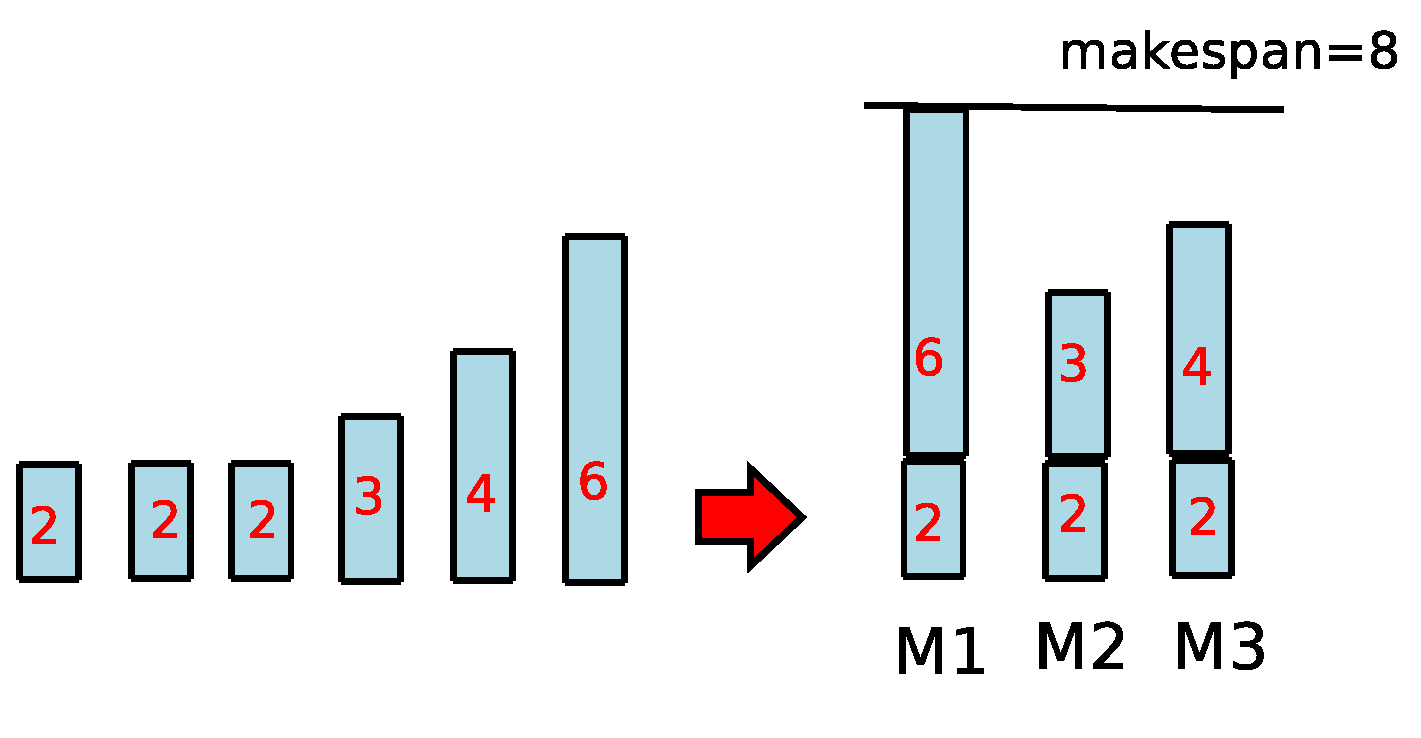
\includegraphics[width=3in]{L11-makespanexample.eps}
    \end{figure}
} 

\frame{
\frametitle{ Problem statement }

   \begin{figure}
        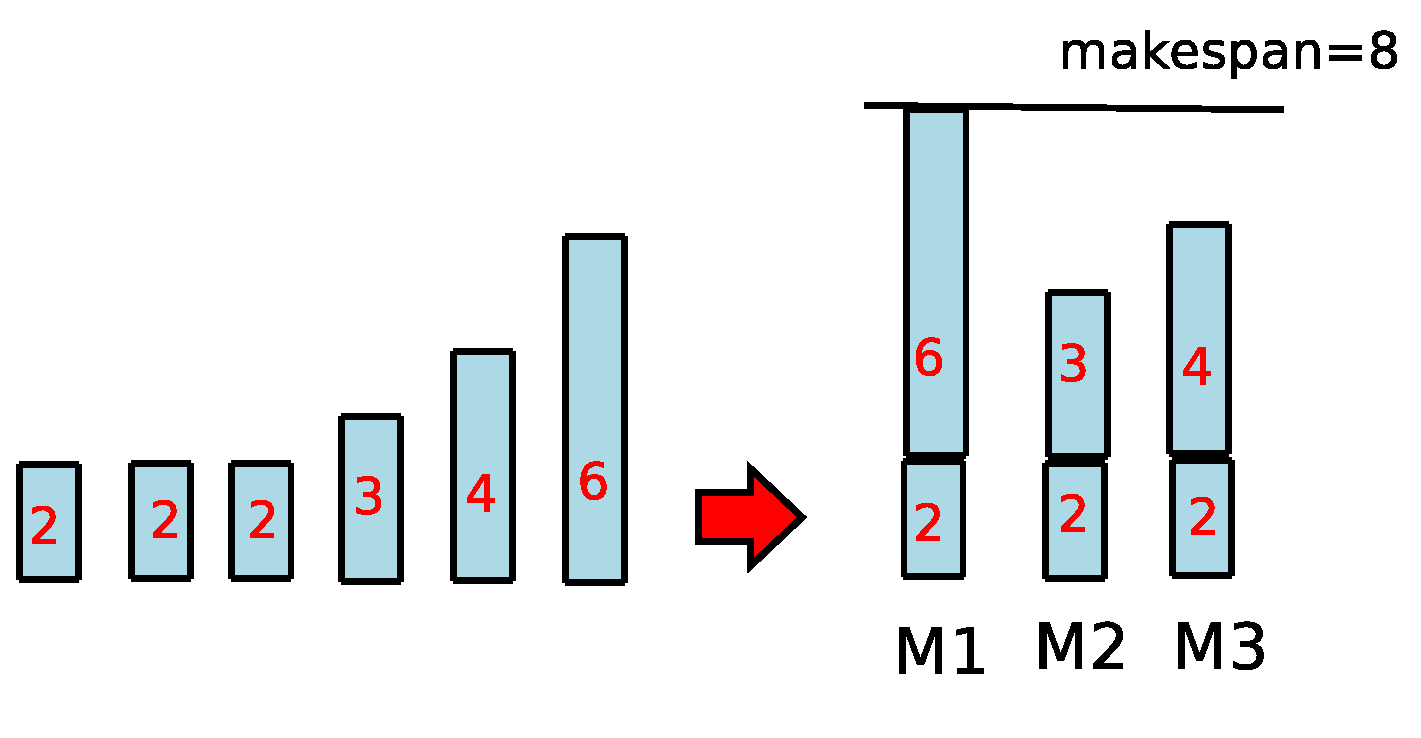
\includegraphics[width=3in]{L11-makespanexample.eps}
    \end{figure}
 
\begin{block}{}
 {\bf INPUT: }  \\ 
$m$ servers $M_1, M_2, ..., M_m$, $n$ jobs (each job $j$ has a processing time $t_j$); 

 {\bf OUTPUT: } \\ 
An assignment of jobs to machines to minimize the {\it makespan }, i.e.  the maximum load on any machine, $T=\max_i \sum\nolimits_{j\in A(i)} t_j$, where $A(i)$ denotes the jobs assigned to machine $i$.
\end{block}

} 

\frame{
\frametitle{ Hardness of {\sc MakeSpan} problem }

\begin{Theorem}
{\sc MakeSpan} is a NP-Complete problem. 
\end{Theorem}
\begin{Proof}
\begin{itemize}  
\item We will prove that {\sc Partition} $\leq_{P}$    {\sc MakeSpan}. 
\item \textbf{Transformation:} 

 Given an instance of {\sc Partition} problem, we construct an instance of {\sc MakeSpan} problem as follows: 
 \begin{enumerate}
  \item For each number $s_i \in S$, new a job $i$ with $t_i = s_i$; 
  \item The objective is to find a schedule of these jobs on $2$ machines with makespan $T=\frac{1}{2} \sum\nolimits_i t_i$. 
 \end{enumerate} 
 \item \textbf{Equivalence:}   It is obvious that a partition corresponds to a schedule. 
\end{itemize} 
\end{Proof}
}


\frame{
\frametitle{ Greedy technique for {\sc MakeSpan} problem }
\begin{itemize}
\item \textbf{Key observation:} solution is a partition of jobs. 
 \item Basic idea: Imagine the solving process as a series of decisions. At each decision step, we assign a job to a machine. 
  Consider a specific job. We have $m$ options.   
 \item Greedy rule: To make loads as balanced as possible, it is reasonable to assign a job to the machine with the smallest load. %\footnote{  In {\sc ShortestPath} problem, an \textcolor{red}{optimal} solution to a subproblem is used to form an \textcolor{red}{optimal} solution to the original problem. Here, a \textcolor{red}{good} solution to the subproblem is used to form a \textcolor{red}{good} solution to the original problem. } 
\end{itemize}
} 

\frame{
\frametitle{ Greedy algorithm}

{\sc GreedyMakeSpan1} algorithm\\
\begin{algorithmic}[1]
\FOR{$i=1$ to $m$}
\STATE $T_i=0$; // $T_{i}$ denotes the load of machine $i$;
\STATE $A_i=\texttt{NULL}$; //initializing all machines with 0 jobs; 
\ENDFOR

\FOR{$j=1$ to $n$}
\STATE Let $k= \arg \min T_i$;
\STATE $A_k= A_k \bigcup \{j\}$; //assigning job $j$ to machine $M_k$
\STATE $T_k = T_k + t_j$;
\ENDFOR
\end{algorithmic}

% 
% \begin{figure}
%         \includegraphics[width=2in]{L11-makespanalgorithm1.eps}
% \end{figure}
} 

\frame{
\frametitle{ An example}
\begin{figure}
      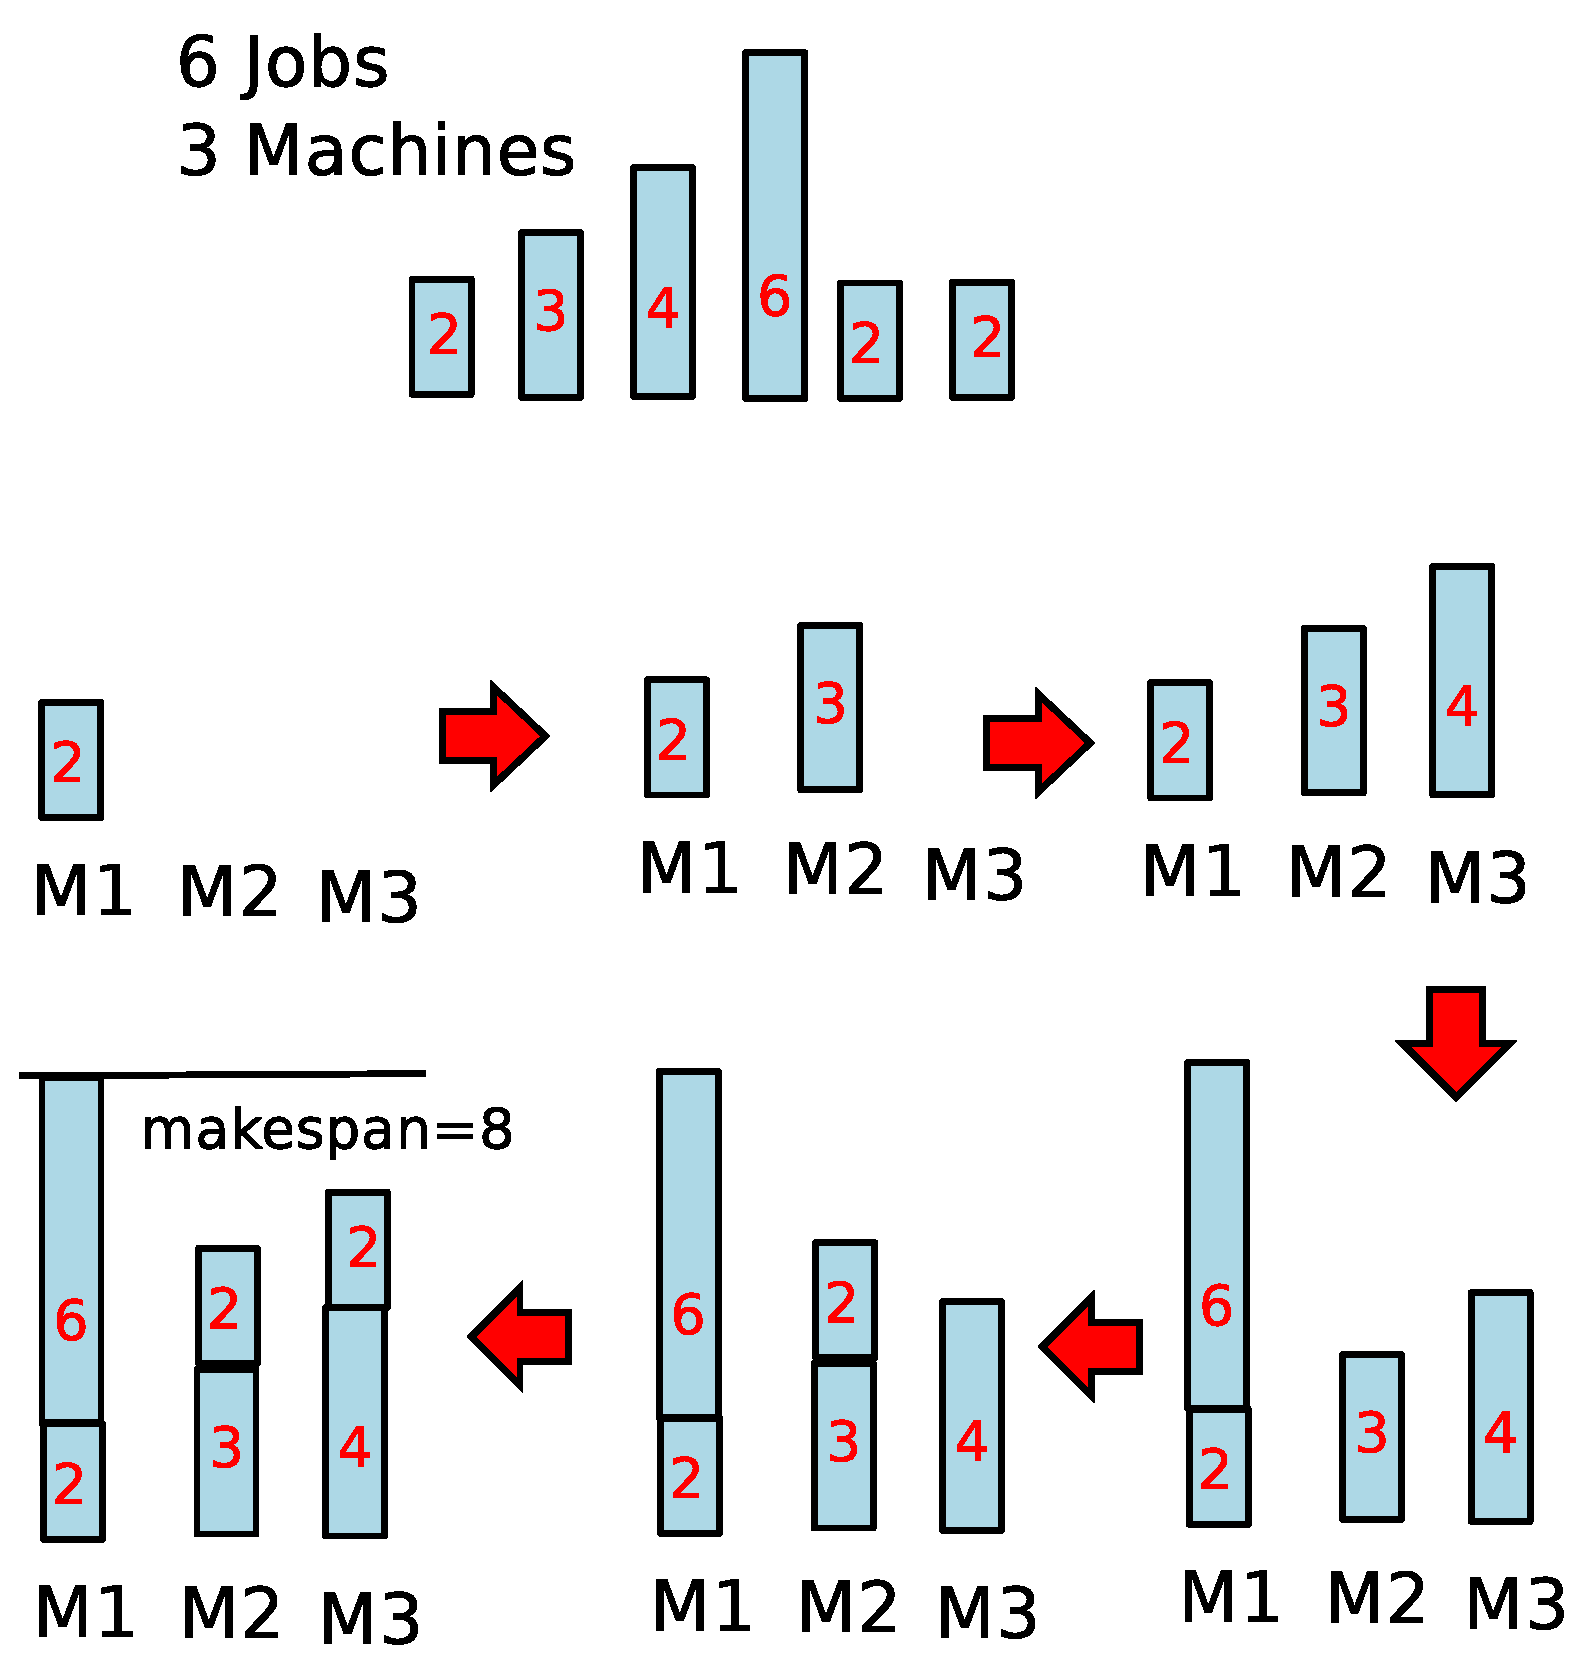
\includegraphics[width=3in]{L11-makespanalgo1example.eps}
\end{figure}
}

\frame{
\frametitle{ Analysis } 
\begin{itemize}
 \item 
Let $T$ be the makespan reported by {\sc GreedyMakeSpan1} algorithm, and $OPT$ be the optimal makespan. 
\item The objective is to measure the quality of $T$ via comparing $T$ with $OPT$. 
\begin{figure}
        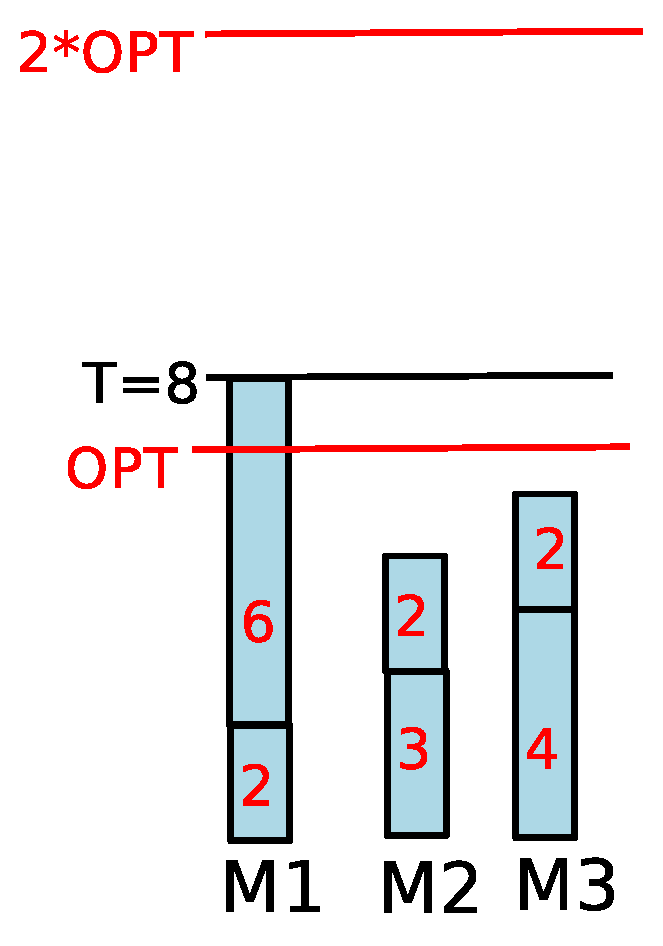
\includegraphics[width=1.2in]{L11-makespanalgo1analysis2OPT.eps}
\end{figure}
\item In the example, {\sc GreedyMakeSpan1} reports $T=8$, which is not too bad since $T$ will not be greater than $2 OPT$.  \end{itemize}
} 

\frame{
\frametitle{ Using a lower bound of $OPT$ rather than $OPT$ itself  } 
\begin{itemize}
\item But how can we compare $T$ against $OPT$ while $OPT$ is yet unknown? 
\item 
Note that though it is difficult to know $OPT$, it is usually easy to obtain a lower bound of $OPT$. 
\item 
Thus we can use the lower bound as a bridge to build connection between $T$ and $OPT$. More specifically, we \textcolor{red}{compare $T$ with the lower bound of $OPT$}  rather than \textcolor{red}{ compare $T$ with $OPT$ directly}. 
\end{itemize}

} 

\frame{
\frametitle{ Finding a lower bound of $OPT$  } 

\begin{itemize}
\item Take {\sc MakeSpan} problem as an example. 
\item Though $OPT$ is unknown, we can easily set lower bound of $OPT$ as follows: 
\begin{enumerate} 
\item Key observation 1: $ OPT \geq \frac{1}{m} \sum\nolimits_j t_j = \frac{19}{3} $. 
\item Key observation 2: $ OPT \geq t_j$ for any $j$; thus, $OPT \geq 6$.   
\end{enumerate}
\end{itemize}
\begin{figure}
        \includegraphics[width=1.4in]{L11-makespanalgo1analysisLB.eps}
\end{figure}
} 

\frame{
\frametitle{ {\sc MakeSpanAlgo1} is not too bad   } 
\begin{itemize}
\item Using the lower bounds as bridge, we can prove the following theorem: 
\begin{Theorem}
$ T \leq 2 OPT $, i.e {\sc GreedyMakeSpanAlgo1} is a $2$-approximation algorithm.
\end{Theorem}
\end{itemize}
\begin{figure}
        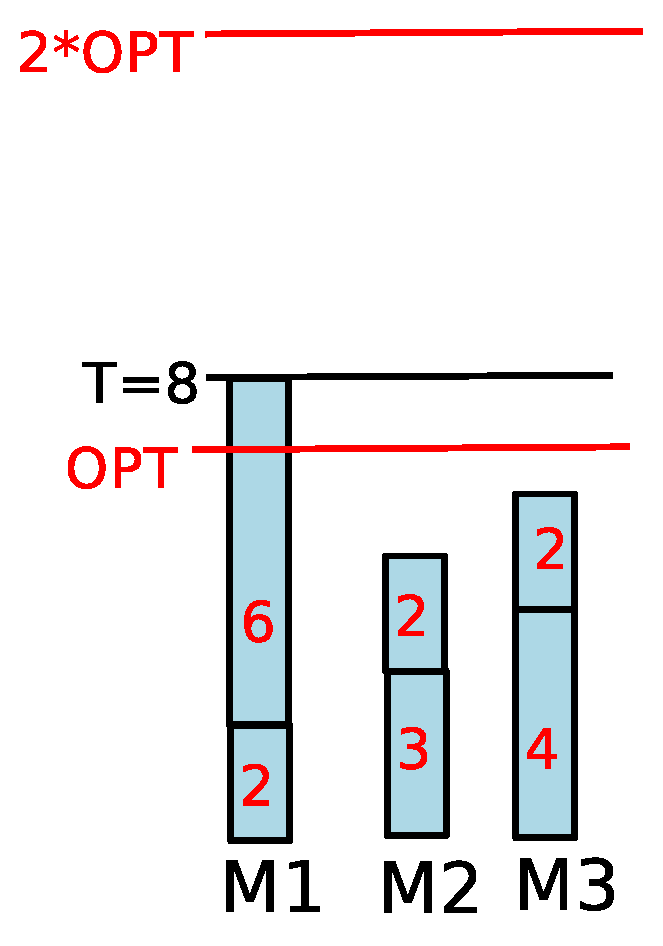
\includegraphics[width=1.2in]{L11-makespanalgo1analysis2OPT.eps}
\end{figure}
} 

\frame{
\begin{Proof}
\begin{itemize}
 \item Let $M_i$ be the machine with the heaviest load $T$; 
 \item Divide $T$ into two parts: the last job $k$, and the previous jobs.Thus  $T=t_k + A $, where $A$ denotes the total load of the previous jobs. 
 \item We have $T \leq 2 OPT$ since
 \begin{enumerate}
 \item $t_k \leq OPT$  (by  observation 2)
  \item $A \leq OPT$.  Why? 
\begin{itemize}
 \item Consider the state whenhe tjob $k$ was assigned to $M_i$. At that time, $M_i$ had a total load of $A$, which is the smallest load of all machines (by the greedy rule of the algorithm). 
 \item Formally, $A  \leq \frac{1}{m} (\sum\nolimits_{j=1}^{n} t_j-t_k) \leq \frac{1}{m} \sum\nolimits_{j=1}^{n} t_j  \leq OPT$ (by key observation 1).
\begin{figure}
        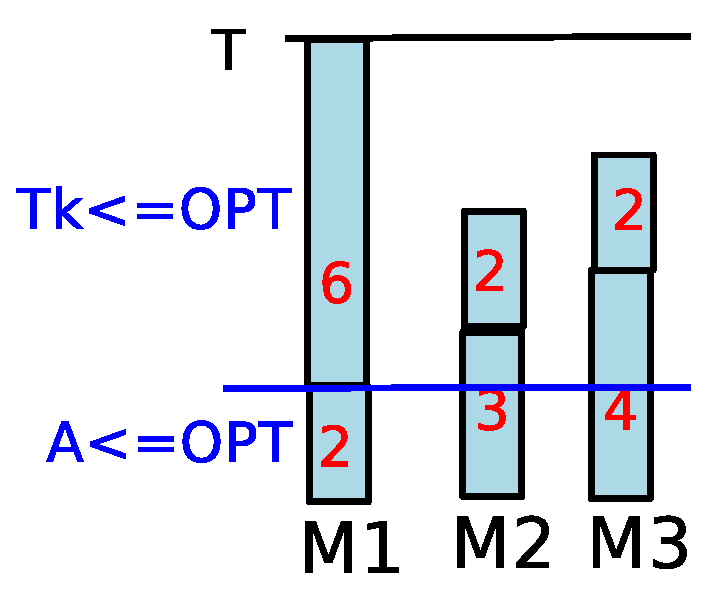
\includegraphics[width=1.5in]{L11-makespanalgo1analysis.eps}
\end{figure}
\end{itemize} 
 \end{enumerate} 
\end{itemize}
\end{Proof}
}

\frame{
\begin{block}{}
Question: is this an accurate analysis? 
\end{block}  
} 

\frame{
\frametitle{ A tight example of {\sc GreedyMakeSpanAlgo1} algorithm}
\begin{itemize}
 \item 
Consider a special instance: a total of $n=m(m-1)+1$ jobs with loads $t_1=t_2=...=t_{n-1}=1$, and $t_n=m$. 
\begin{figure}
        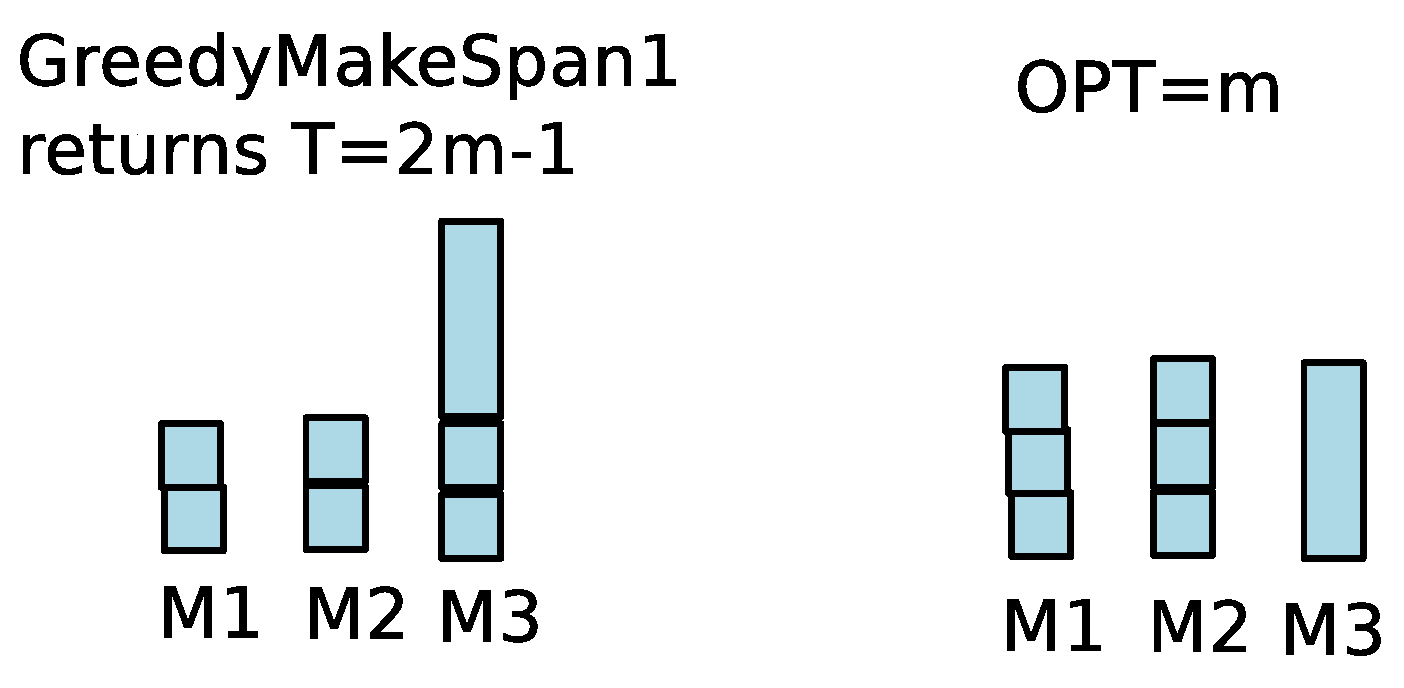
\includegraphics[width=2.8in]{L11-makespanalgo1tightexample.eps}
\end{figure}
 \item 
 {\sc GreedyMakeSpan1}: $T=2m-1$ (if the largest job $n$ is processed at the last step). 
\item OPT: $OPT=m$.  
 \item 
Thus, approximation factor is:  $\alpha  = \frac{ T } {  OPT}  = 2- \frac{1}{m}$. $\alpha$ can be arbitrarily close to $2$ when $m$ increases. 
\end{itemize}



} 

\frame{
\begin{block}{}
Another greedy algorithm for {\sc MakeSpan} 
\end{block}  
} 

\frame{
\frametitle{Basic idea } 
\begin{itemize}
 \item 
Basic idea: The tight example for {\sc GreedyMakeSpanAlgo1} algorithm implies that it is not wise to process the largest job finally. In other words, it might be a good idea to process large jobs first.
\end{itemize}
\begin{figure}
    \includegraphics[width=4in]{L11-makespanalgo2example.eps}
\end{figure}
} 

\frame{
\frametitle{Another greedy algorithm } 
  {\sc GreedyMakeSpan2} algorithm\\
\begin{algorithmic}[1]
\FOR{$i=1$ to $m$}
\STATE  $T_i=0$;  //assigning all machines with 0 jobs; 
\STATE $A_i=\texttt{NULL}$;
\ENDFOR
\STATE \textcolor{red}{\bf sort jobs in decreasing order of $t_j$;} //process large jobs first
\FOR{$j=1$ to $m$}
\STATE Let $k= argmin\ T_i$; //assign job $j$ to $M_k$;
\STATE $A_k= A_k \bigcup \{j\}$;
\STATE $T_k = T_k + t_j$;
\ENDFOR
\end{algorithmic}

}

\frame{
\frametitle{Analysis } 
\begin{itemize}
\item \textbf{Key observation 3:} $ OPT \geq 2 t_{j}$ for any $j \geq m+1$ if all jobs were sorted decreasingly. \\
(Why? Consider the first $m+1$ jobs only. At least two jobs should be assigned to a machine. Thus, $OPT \geq 2 t_{m+1}$. ) 
\end{itemize}
\begin{figure}
    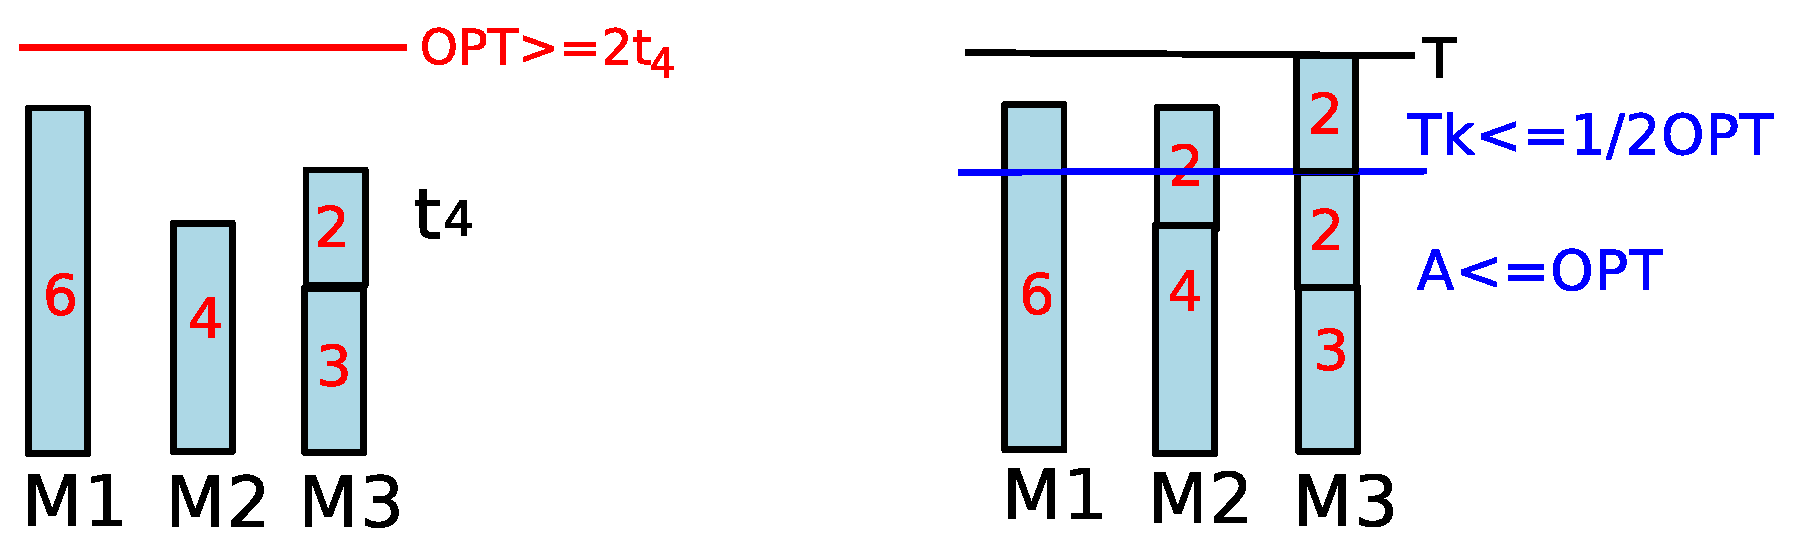
\includegraphics[width=4in]{L11-makespanalgo2analysis.eps}
\end{figure}
} 


\frame{
\frametitle{Analysis} 

\begin{Theorem}
$ T \leq 1.5 OPT $, i.e, {\sc GreedyMakeSpanAlgo2} is a $1.5$-approximation algorithm.
\end{Theorem}
\begin{Proof}
\begin{itemize}
 \item Let $M_i$ be the machine with the heaviest load $T$ reported by {\sc GreedyMakeSpanAlgo2} algorithm; 
 \item Divide $T$ into two parts: the last job $k$, and the previous jobs. Thus $T=t_k + A $, where $A$ denotes the total load of the previous jobs.

 \item $T \leq 1.5 OPT$ since:
 \begin{enumerate}
  \item $t_k \leq \frac{1}{2} OPT$  (by  observation 3)
  \item $A \leq OPT$ (the same argument to the last theorem)
 \end{enumerate} 
\end{itemize}
 \end{Proof}
}

\frame{
\begin{block}{}
 The key steps in approximation algorithm  design
\end{block}
}

\frame{
\frametitle{A dilemma}
\begin{itemize}
\item We are facing a dilemma: 
 \begin{enumerate}
  \item In order to establish the approximation guarantee, we should compare the quality of a solution against the quality of the optimal solution $OPT$. 
\item However, it is NP-Hard to compute  the optimal solution value $OPT$ and to find an optimal solution.
\end{enumerate}
\item Question:  How can we establish the connection with $OPT$ \textcolor{red}{\bf without} the exact value of  $OPT$?
\item   The answer to this question provides a key step in the design of approximation algorithms. 
\end{itemize}

} 

\frame{
\frametitle{The key step in approximation algorithm  cont'd }

\begin{itemize}
\item {\bf  Strategy:} Finding a lower bound of $OPT$ and  \textcolor{red}{\bf  comparing a solution with the lower bound} rather than  \textcolor{red}{\bf comparing with $OPT$ directly!  } 

 \item \textbf{Key step 1:}  Although it is NP-Hard to find optimal solution, it might be polynomial-time computable to find a \textcolor{red}{\bf ``tight lower bound''} of $OPT$.  
 \item \textbf{Key step 2:} We should figure out a process to yield a feasible solution, and compare this solution with the lower bound of OPT. 
\end{itemize}

} 

\frame{
\frametitle{Finding a lower bound } 
 
\begin{itemize}
\item Then how to find a lower bound of $OPT$? 
\begin{enumerate}
 \item Combinatorial ways: problem specific and thus cohesive; then we design greedy or DP algorithm; 
 \item LP-based method as a united way: LP-relaxation, duality, etc.
\end{enumerate}
\end{itemize}
}


\frame{
\begin{block}{}
 Another example: {\sc Set Cover} problem
\end{block}
}

\frame{
\frametitle{ {\sc Set Cover} problem}
\begin{itemize}
 \item
Practical problems: 
\begin{itemize}
 \item An anti-virus package identifies a viruses based on characteristic ``keywords'' set, and a keyword corresponds to several viruses. The question is how to select a small ``representative'' keywords set to detect all viruses. 
 \item To form a committee, containing as few people as possible, to cover all requisite skills; 
 \end{itemize}
 \end{itemize}
} 

\frame{
\frametitle{ {\sc Set Cover} problem: formulation }

\begin{block}{Formalized Definition:} 
{\bf INPUT:} a set of $n$ elements $U=\{1,2,...,n\}$,  and $m$ subsets of $U$, denoted as  $S_1, S_2,...,S_m$. \textcolor{red}{Each subset $S_i$ has a weight $w_i$.}  \\
{\bf OUTPUT:} to find a collection of subsets, with the minimal weight sum, such that all elements of $U$ are covered.
\end{block}

Note: {\sc SetCover} problem plays an important role in approximation algorithm design as {\sc Matching} problem in the design of exact algorithm.
 
}

\frame{
\frametitle{ An example }

\begin{figure}
 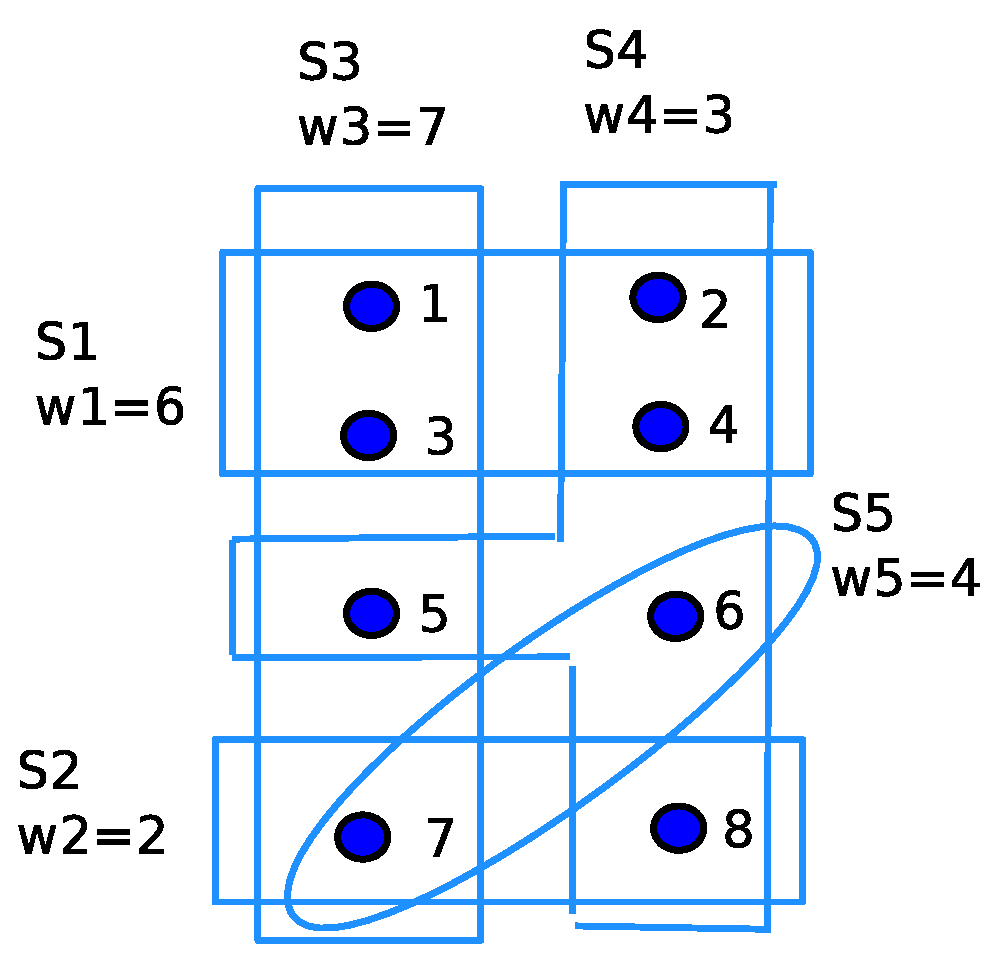
\includegraphics[width=2.2in]{L11-setcoverexamplelognstep1.eps}
\end{figure}
\begin{itemize}
\item 
Question: how to choose several subsets, with the minimal weight sum, such that all elements are covered?
\end{itemize} 
}

 
\frame{
\frametitle{Greedy algorithm} 
\begin{itemize}
\item \textbf{Key observation:} solution is a collection of subsets. Imagine the solving process as a series of decisions. At each decision step, we decide to choose a subset or abandon it.   
\item {\bf Greedy selection rule:} we should consider two aspects of a subset:
\begin{enumerate}
\item  the smaller the weight, the better; 
\item the more items it covers, the better. 
\end{enumerate}
Thus, it is reasonable to select a subset based on \textcolor{red}{\bf ``the ratio of weight over the number of items it covers''}. 
\end{itemize} 
} 

\frame{ 
\frametitle{Greedy algorithm} 
{\sc Greedy-Set-Cover} algorithm\\
\begin{algorithmic}[1]
\STATE $I=\texttt{NULL}$; //$I$ denotes the index of selected subsets; 
\STATE $R=U$; // $R$ denotes the remaining elements; 
\WHILE{$R \neq \texttt{NULL}$}
\STATE $j = \arg \min_i \frac{w_i}{ |S_i \cap R | }$; 
\STATE  \textcolor{blue} { Let $p_j= \frac{w_j}{ |S_j \cap R | } $;}
\FORALL{ \textcolor{blue} { remaining element $e \in R \cap S_j$} } 
\STATE  \textcolor{blue} { Set $price(e) = p_j$; }
\ENDFOR
\STATE $I=I \cup \{j\}$;
\STATE $R= R - S_j$;
\ENDWHILE
\end{algorithmic}
% \begin{figure}
%  \includegraphics[width=1.8in]{L11-setcoveralgorithm4.eps}
% \end{figure}
} 

\frame{
\frametitle{An example: Step 1}
\begin{figure}
 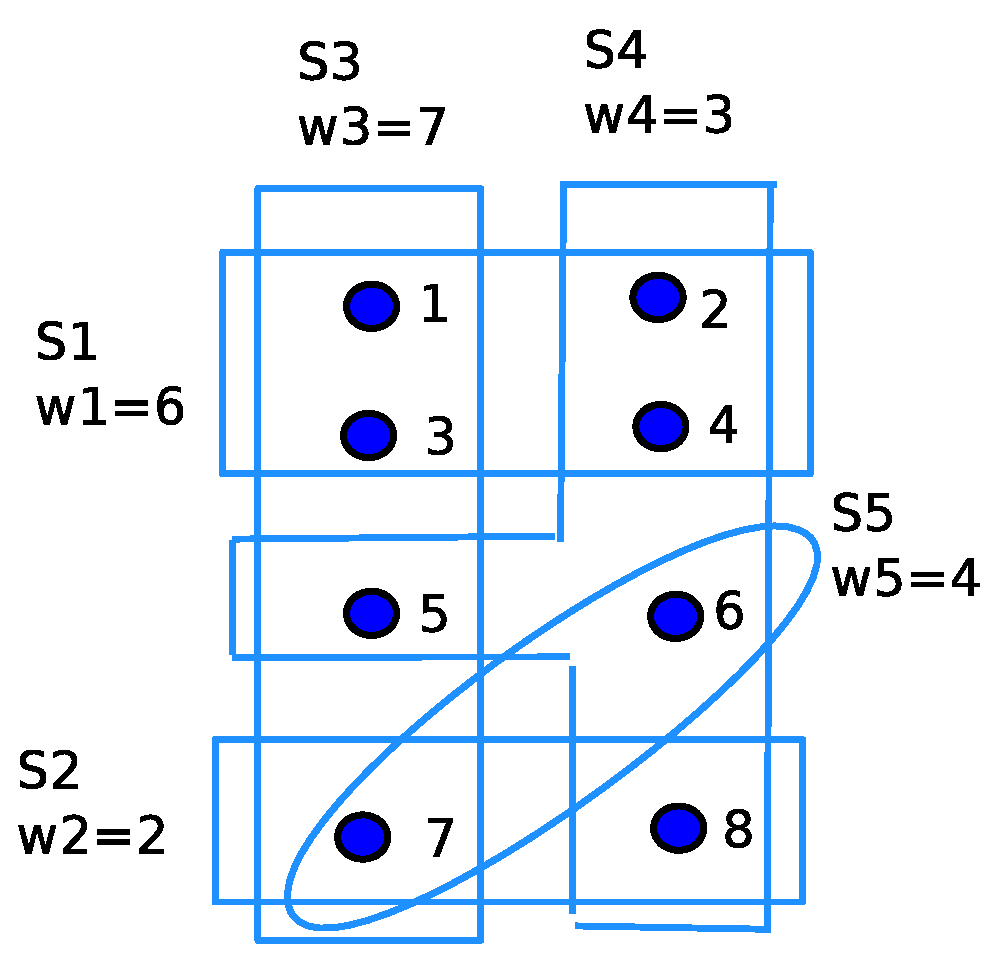
\includegraphics[width=2in]{L11-setcoverexamplelognstep1.eps}
\end{figure}

Step 1: 
\begin{itemize} 
\item $R=U=\{1,2,3,4,5,6,7,8\}$; \\
\item           $p_1=\frac{w_1}{|S_1\cap R|}=\frac{6}{4};$ \  $p_2=\frac{w_2}{|S_2\cap R|}=\frac{2}{2};$ \   $p_3=\frac{w_3}{|S_3\cap R|}=\frac{7}{4};$ \   $p_4=\frac{w_4}{|S_4\cap R|}=\frac{3}{5}; $ $p_5=\frac{w_5}{|S_5\cap R|}=\frac{4}{2};$ \\ 
\item 	  
          Choose $S_4$ since $p_4$ is the smallest one.
\end{itemize}
} 

\frame{
\frametitle{An example: Step 2}
\begin{figure}
 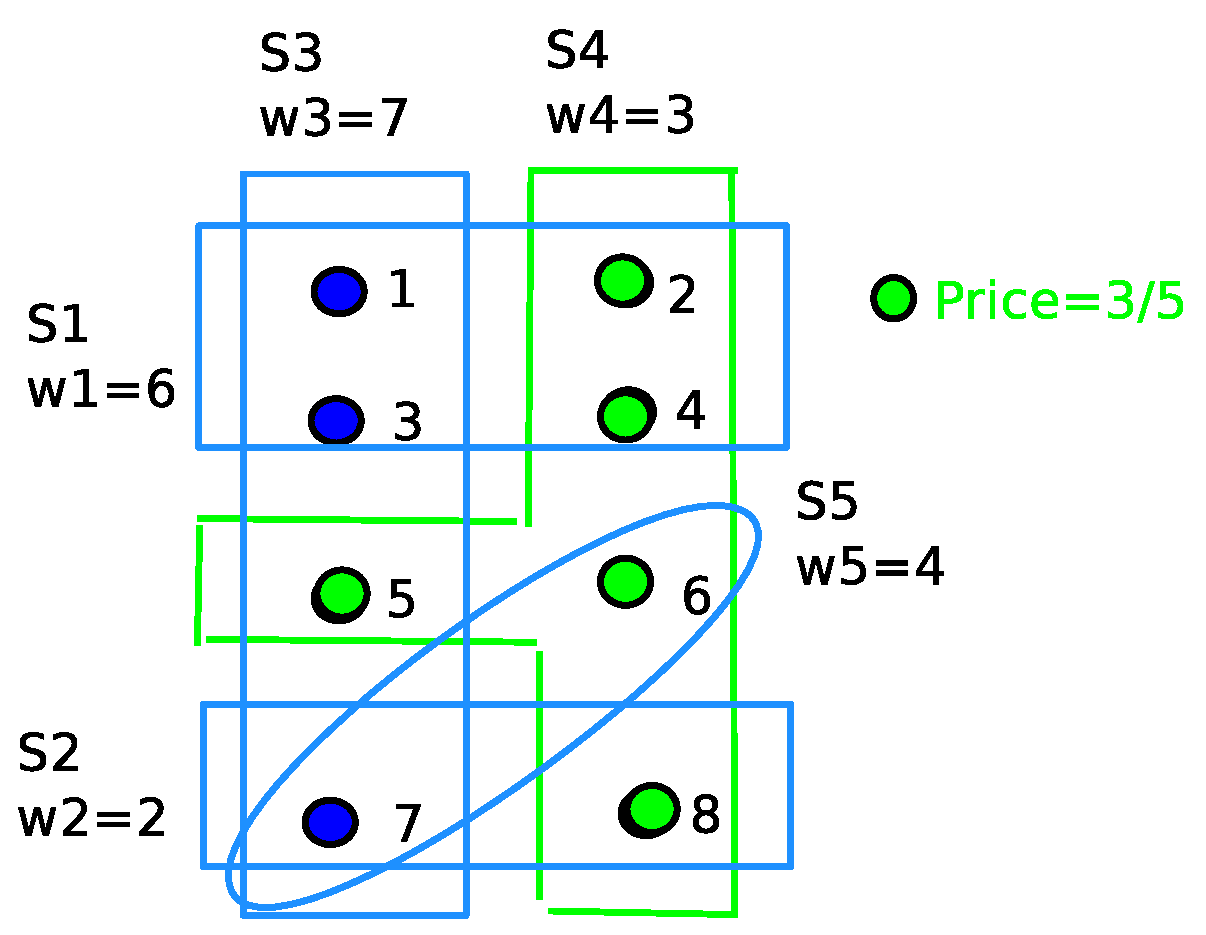
\includegraphics[width=2.8in]{L11-setcoverexamplelognstep2.eps}
\end{figure}

Step 2: \begin{itemize} 
\item $R=\{1,3,7\}$; \\
\item  $p_1=\frac{w_1}{|S_1\cap R|}=\frac{6}{2};$ \  $p_2=\frac{w_2}{|S_2\cap R|}=\frac{2}{1};$ \   $p_3=\frac{w_3}{|S_3\cap R|}=\frac{7}{3};$ \ $p_5=\frac{w_5}{|S_5\cap R|}=\frac{4}{1}$;  \\ 

   \item        Choose $S_2$ since $p_2$ is the smallest one.
\end{itemize}
} 

\frame{
\frametitle{An example: Step 3}
\begin{figure}
 \includegraphics[width=2.8in]{L11-setcoverexamplelognstep3.eps}
\end{figure}

Step 3: \begin{itemize} 
\item $R=\{1,3\}$; \\
       \item  $p_1=\frac{w_1}{|S_1\cap R|}=\frac{6}{2};$ \  $p_3=\frac{w_3}{|S_3\cap R|}=\frac{7}{2};$ 
 	
        \item   Choose $S_1$ since $p_1$ is the smallest one. 
\end{itemize}
} 

\frame{
\frametitle{An example: Step 4}
\begin{figure}
 \includegraphics[width=2.8in]{L11-setcoverexamplelognstep4.eps}
\end{figure}

Step 4: \begin{itemize} 
\item $R=\{\}$. Done! \\

\item Solution: We select $I=\{S_1, S_2, S_4\}$ with the sum of weight: 11. 

\item Optimal solution: selecting $\{ S_3, S_4\}$ with the sum of weight: 10.
\end{itemize} 
}

\frame{
\frametitle{Performance analysis }
\begin{itemize} 
\item 
We will prove the following theorem: 
\end{itemize}
\begin{Theorem}
 {\sc Greedy-Set-Cover} algorithm is an $H(f)$-approximation algorithm, where $f=\max_i |S_i|$. 
\end{Theorem}
\begin{itemize} 
\item 
Meaning:  The algorithm returns a subset $I=\{S_1, S_2, S_4\}$ with the total weight of 11. We guarantee that $W=11 \leq H(5) OPT = H(5) 10$. 
\end{itemize} 
} 

\frame{ 
\frametitle{} 
\begin{Proof}
Let $S^*$ be the optimal solution, and $S$ be the solution returned by {\sc Greedy-Set-Cover} algorithm. We have:  
\begin{eqnarray} 
\sum_{S_i \in S } w_i  &=& \sum_{e \in U } price(e) \text{ \quad (by Line 7-9)} \\ 
                       &\leq& \sum_{S_j \in S^*} \sum_{e \in S_j}  price(e) \text{ \quad (by S* covers U) } \\ 
		       &\leq& \sum_{S_j \in S^*} H( |S_j| ) w_j   \text{ \quad (by the lemma) }  \\ 
		       &\leq& \sum_{S_j \in S^*} H( f ) w_j \text{ \quad ($d$ is the largest)} \\
		       &=& H( f ) OPT 
\end{eqnarray}
\end{Proof}
}

 


\frame{
\frametitle{Finding a lower bound}


\begin{lemma}
 For each subset $S_i$, $\sum_{e \in S_i} price(e) \leq H(|S_i|) w_i$. 
\end{lemma}

\begin{itemize}
\item 
Take $S_1$ as an example. We have: 
\begin{eqnarray}
\Sigma _{e \in S_1} price( e ) & = & ( \frac{w_4}{5}  + \frac{w_4}{5} )  + (\frac{w_1}{2}  + \frac{w_1}{2} ) \\
& \leq & ( \frac{ w_1 }{4} + \frac{ w_1 }{4} ) + ( \frac{ w_1 }{2} + \frac{ w_1 }{2} ) \\
& \leq & ( \frac{ w_1 }{4} + \frac{ w_1 }{3} ) + ( \frac{ w_1 }{2} + \frac{ w_1 }{1} ) \\
& = & w_1 H(4) \nonumber
\end{eqnarray}
\item Here,  the first $\leq$ is due to the selecting criteria in Step 2, i.e. $p_4 = \frac{w_4}{5}$ is smaller than $p_1 = \frac{ w_1 }{4}$, and the selecting criteria in Step 3, i.e. $p_1 = \frac{ w_1 }{2} $ is smaller than $p_3 = \frac{ w_3}{2}$.
\end{itemize}
} 


\frame{
\begin{block}{}
Question: is this an accurate analysis? 
\end{block} 
} 

\frame{
\frametitle{ A tight example }

\begin{itemize}
 \item 
 Consider a special instance: $n+1$ subsets with weights $\frac{1}{n}, \frac{1}{n-1}, ..., \frac{1}{2}, 1$ and $1+\epsilon$, respectively. 
\begin{figure}
 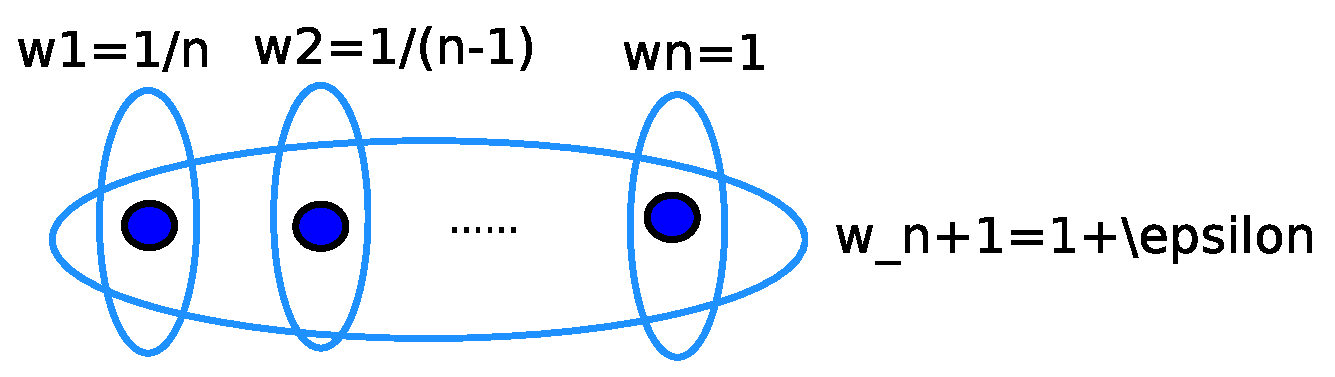
\includegraphics[width=3.5in]{L11-setcoveralgo4tightexample.eps}
\end{figure}
 \item Optimal solution: selecting only one subset with weight $1+\epsilon$; 
 \item {\sc Greedy-Set-Cover} result: selecting $n$ subsets with the sum of weight $\frac{1}{n} + \frac{1}{n-1} + ... + \frac{1}{2} + 1 = H(n)$. 
\end{itemize}
}

\frame{
\begin{block}{}
 LP as a unified approach framework to lower bound $OPT$
\end{block}
}

\frame{
\begin{block}{}
Lower bound 1: $z_{LP} \leq z_{ILP} = OPT$
\end{block}
}


\frame{
\frametitle{LP as a unified framework: Step 1 }

\begin{itemize} 
\item 
\textbf{Step 1: } Formulate the problem as an integer linear program (ILP);\\

\item 
We define a 0/1 variable $x_j$ for each subset $S_j$, where $x_j = 1$ means the selection of $S_j$, and 0 means abandon. \\
\item ILP model: 
\[
\begin{array}{lllllllll}
 \min&  z=& \sum\nolimits_{j=1}^m w_j x_j \\
 s.t.&  & \sum\nolimits_{j: e \in s_j} x_j & \geq 1 & \forall e \in U \\ 
     &  & \textcolor{red}{x_j}                   & \textcolor{red}{= 0/1 } & \forall i 
\end{array} \nonumber
\]
\item Thus we have $OPT=z_{ILP}$, where $z_{ILP}$ denotes the optimal objective value of the ILP model. 
\end{itemize} 
} 


\frame{
\frametitle{LP as a unified approach framework: Step 2 }
\begin{itemize} 
\item 
\textbf{Step 2:}  Relaxing ILP into LP;  \\
\item LP relaxation: 
\[
\begin{array}{llllll}
 \min &z=& \sum\nolimits_{j=1}^m w_j x_j \\
 s.t. & &\sum\nolimits_{j: e \in s_j} x_j & \geq  1 & \forall e \in U \\ 
             &  &  \textcolor{red}{x_j}  &\textcolor{red}{\geq 0} &  \forall i  \\
      &  &  \textcolor{red}{x_j}  &\textcolor{red}{\leq 1} &  \forall i  \\
\end{array} \nonumber
\]
\item \textcolor{red}{Key observation 1: } $z_{LP} \leq z_{ILP} = OPT$, where $z_{LP}$ denotes the optimal objective value of the LP model. \\
\end{itemize} 
} 

\frame{
\frametitle{LP as a unified approach framework: Step 3 }

\begin{itemize} 
\item 
\textbf{Step 3: } Since the LP model might generate a fractional solution, a clever way should be figured out to transform the \textcolor{red}{optimal solution to LP} (in polynomial-time) to  \textcolor{red}{a feasible solution to ILP}, whose objective value is close to \textcolor{red}{the optimal LP objective value}.  
\item 
The final difficulty: how to obtain a feasible solution to ILP based on the optimal solution to LP? \textcolor{red}{\bf Rounding! }
\end{itemize} 
}

\frame{
\frametitle{Algorithm1: LP+Rounding} 


 
LP+Rounding algorithm\\
\begin{algorithmic}[1]
\STATE Solve the linear program $LP$ to get an optimal solution $x^*$; 
\STATE $I=\texttt{NULL}$;
\FORALL{ subset $S_j$}
\IF{$x_j^* \geq \frac{1}{f} $}
\STATE $I = I + \{j\}$;
\ENDIF
\ENDFOR
\RETURN $I$;
\end{algorithmic}

% \begin{figure}
%  \includegraphics[width=3.5in]{L11-setcoveralgorithm1.eps}
% \end{figure}
\begin{itemize} \item Here  $d$ denotes the largest coverage of any element in $U$, i.e.  $d=\max_{e \in U} |\{ j: e \in S_j\}|$. 
\end{itemize} 
} 

\frame{
\frametitle{An example }
\begin{figure}
 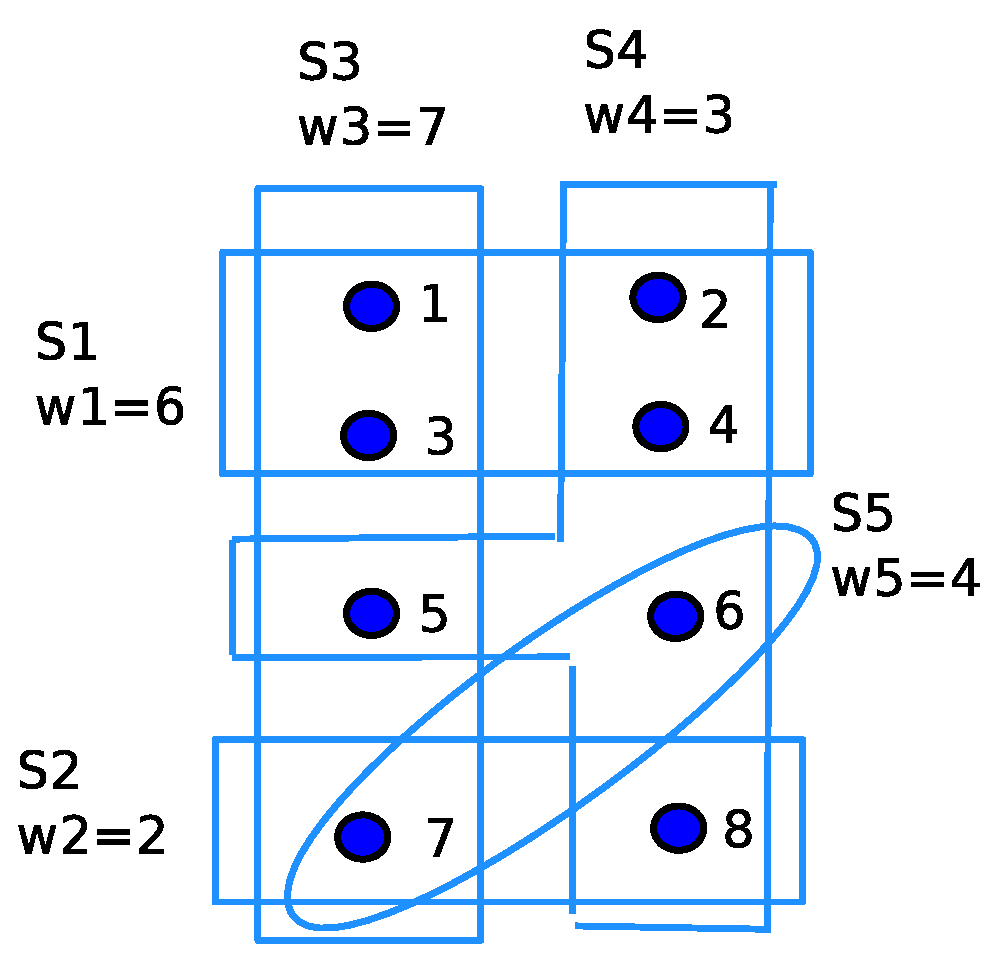
\includegraphics[width=1.1in]{L11-setcoverexamplelognstep1.eps}
\end{figure}
\begin{scriptsize}
\[
\begin{array}{rrrrrrrrrrrr}
 \min & 6x_1   &+& 2 x_2   &+& 7 x_3    &+& 3 x_4    &+& 4 x_5     &           & \\
 s.t. & x_1    & &         &+&     x_3 & &         & &         & \geq 1    & \text{(item 1,3)} \\
      &   x_1  & &         & &         &+&    x_4  & &         & \geq 1   & \text{(item 2,4)}\\
      &        & &         & &    x_3  &+&    x_4  & &         & \geq 1   & \text{(item 5)}\\
      &        & & x_2     & &         & &         &+&     x_5 & \geq 1   & \text{(item 6)}\\
      &        & & x_2     &+&  x_3    & &         &+&     x_5 & \geq 1   & \text{(item 7)}\\
      &        & & x_2     & &         &+& x_4     & &         & \geq 1   &\text{(item 8)}\\
      &        & &         & &         & &         & &   x_i   & \geq 0   &         \\
      &        & &         & &         & &         & &   x_i   & \leq 1   &         \\	
\end{array} \nonumber
\] 
\begin{itemize}
\item 
LP optimal solution: $x_1=0.5$; $x_2=1$; $x_3=0.5$; $x_4=0.5$; $x_5=0$; 
\item 
Objective  value of  $LP$: 10. ($z_{LP} \leq z_{ILP} = OPT$.)
\item 
Rounding solution: $x'_1 = 1$; $x'_2 = 1$; $x'_3 = 1$; $x'_4 = 1$; $x'_5 = 0$; 
\item 
Objective  value: $18 \leq  d \times  z_{LP}  $.
\end{itemize} 
\end{scriptsize}
}

\frame{
\frametitle{Correctness of Algorithm1 }
\begin{Theorem}
 Algorithm1 yields a set cover. 
\end{Theorem}
\begin{Proof}
(by contradiction)
\begin{itemize}
 \item Suppose there is an element $e$ not covered, i.e.  $e \notin \cup_{j \in I} S_j$. 
 \item Then for each $S_j$ that contains $e$ as a member, we have $x_j^* < \frac{1}{f}$; (Otherwise, $S_j$ should be selected by Algorithm1.)
 \item Thus, $\sum\nolimits_{j: e \in S_j} x_j^* < \frac{1}{d} | \{j: i \in S_j\} | \leq 1$. 
 \item A contradiction against the linear program constraints.
\end{itemize}
\end{Proof}
}

\frame{
\frametitle{Analysis of Algorithm1}
\begin{Theorem}
 (Hochbaum '82) Algorithm1 is an $f$-approximation algorithm for {\sc SetCover}. 
\end{Theorem}
\begin{footnotesize}
 
\begin{Proof}
 \begin{itemize}
  \item Algorithm1 returns a collection $I$ with cost: $C=\sum\nolimits_{j \in I} w_j$;  \begin{eqnarray}
         C &=& \sum\nolimits_{j \in I} w_j  \nonumber \\ 
	   &\leq& \sum\nolimits_{j \in I} w_j x_j^* d \nonumber \\
	   &\leq& \sum\nolimits_{j=1}^m w_j x_j^* d \nonumber  \\ 
	   &=& d \sum\nolimits_{j=1}^m w_j x_j^* \nonumber  \\ 
	   &=& d z_{LP} \nonumber \\ 
	   &\leq& f OPT \nonumber 
        \end{eqnarray}
\item 
  Here, the first inequality follows due to the ``rounding criteria'', i.e.   $x_j^* \geq \frac{1}{d}$.
\end{itemize}
\end{Proof}
\end{footnotesize}
}

\frame{
\begin{block}{}
Lower bound 2: $z_{Dual} \leq z_{LP} \leq z_{ILP} = OPT$
\end{block}
}

\frame{
\frametitle{Algorithm2: Dual LP + Rounding } 

\begin{itemize} 
\item 
Basic idea: rounding the dual solution. 

\item 
Dual: 
\[
\begin{array}{rrrrrrrrl}
 \max d=& \sum\nolimits_{e \in U} y_e &  \\
 s.t. & \sum\nolimits_{e: e \in S_j} y_e  & \leq & w_j & \forall S_j  \\ 
      & y_e                                                 & \geq&  0  & \forall e \in U 
\end{array} \nonumber
\]
\end{itemize} 
} 

\frame{
\frametitle{ Dual provides another lower bound } 

\textbf{Key observation 2:} $\sum_e y_e \leq z_{LP} \leq OPT$ for any feasible dual solution $y$; 

\begin{figure}
 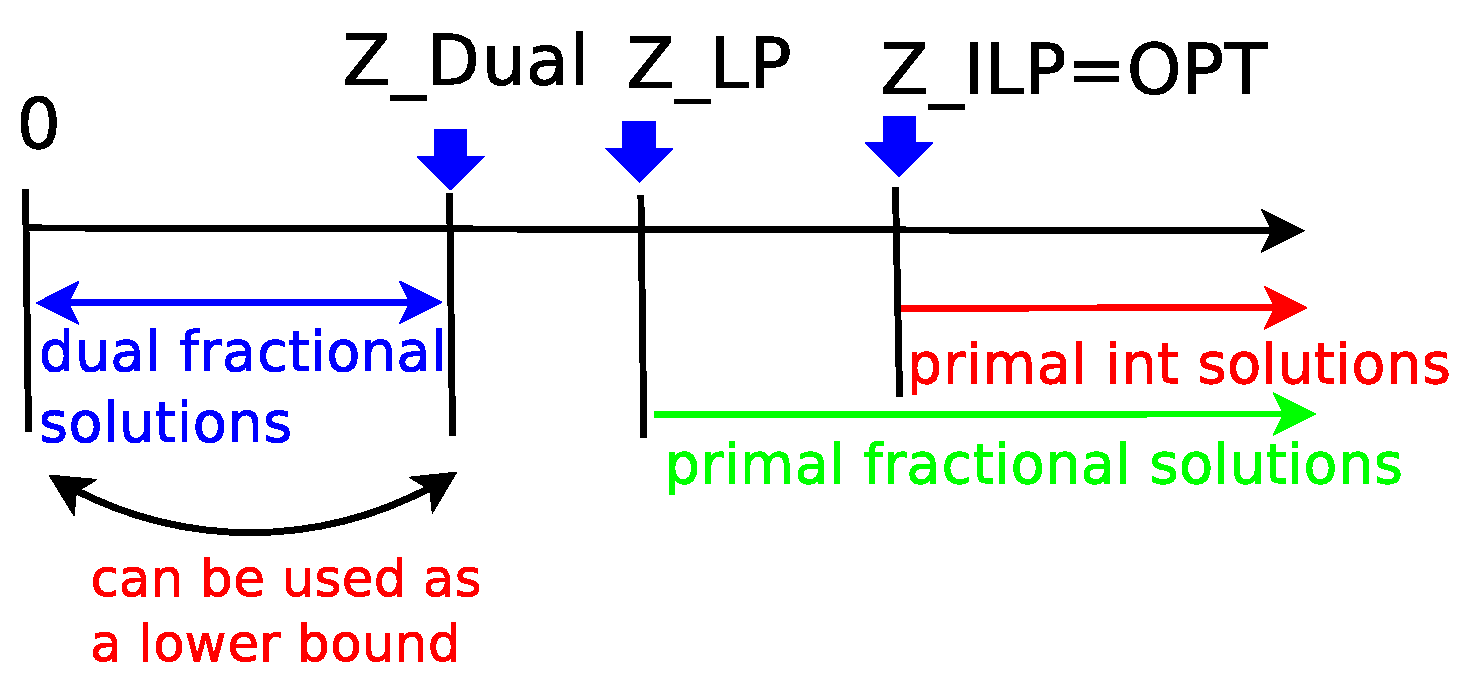
\includegraphics[width=2.5in]{L11-LPlowerbounding.eps}
\end{figure}
} 


\frame{
\frametitle{Algorithm2: Dual LP + Rounding } 

Dual LP + Rounding Algorithm\\
\begin{algorithmic}[1]
\STATE Solve the dual $LP$  to get an optimal solution $y^*$;
\STATE $I=\texttt{NULL}$;
\FORALL{ subset $S_j$}
\IF{$\sum_{e: e \in S_j} y_e^* = w_j$}
\STATE $I = I + \{j\}$;
\ENDIF
\ENDFOR
\RETURN $I$;
\end{algorithmic}
}


\frame{
\frametitle{An example }

\begin{figure}
 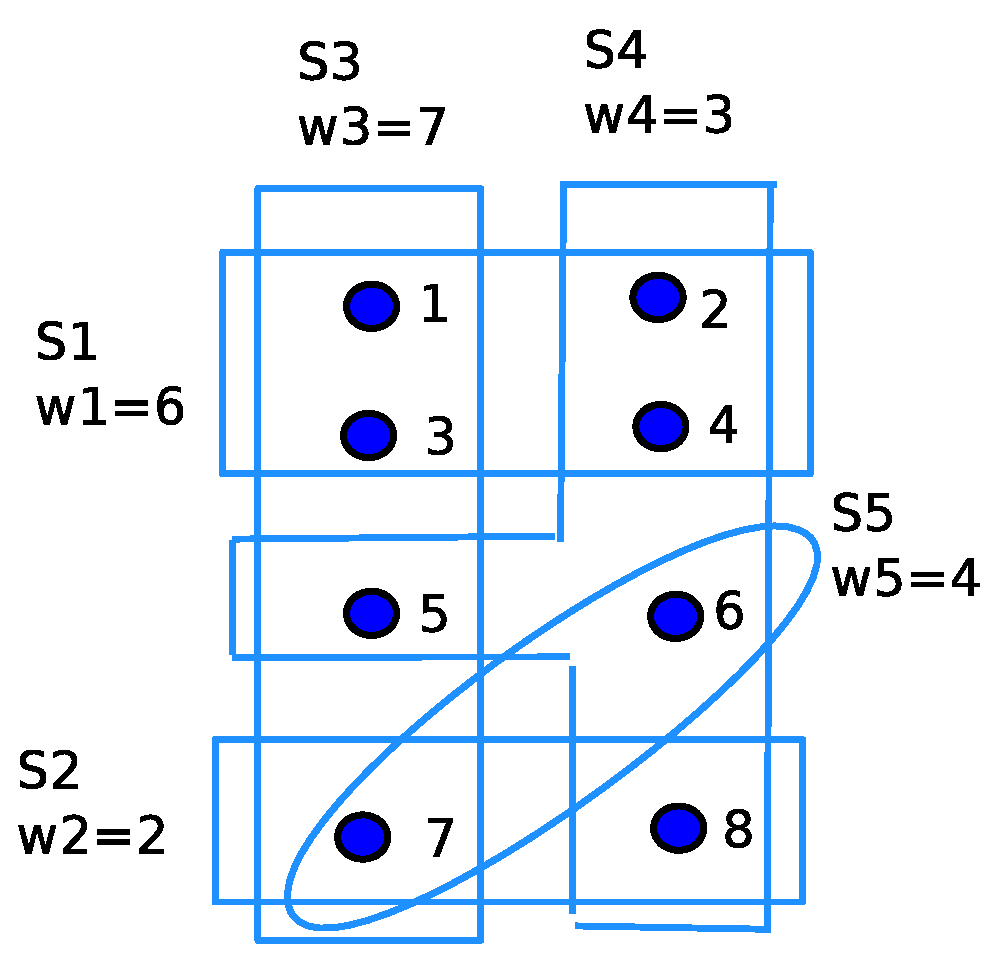
\includegraphics[width=1.2in]{L11-setcoverexamplelognstep1.eps}
\end{figure}

\begin{scriptsize}
\[
\begin{array}{rrrrrrrrrrrrrrrrrr}
 \max& y_1   &+&  y_2   &+& y_3    &+& y_4    &+& y_5  &+&  y_6   &+& y_7  &+& y_8  & \\
 s.t.& y_1   &+&  y_2   &+& y_3    &+& y_4    & &      & &        & &      & &      & \leq 6  \\
     &       & &        & &        & &        & &      & &        & & y_7  &+& y_8  & \leq 2  \\
     & y_1   & &        &+& y_3    & &        &+& y_5  & &        &+&  y_7 & &      & \leq 7  \\
     &       & & y_2    & &        &+& y_4    &+& y_5  &+& y_6  & &      &+&  y_8 & \leq 3  \\
     &       & &        & &        & &        & &        & & y_6  &+&  y_7 & &      & \leq 4  \\
     &       & &        & &        & &        & &        & &      & &      & &  y_i & \geq 0  \\
\end{array} \nonumber
\] 

\begin{itemize} 
\item 
Dual LP optimal solution: $y_1=6$; $y_2=0$; $y_3=0$; $y_4=0$; $y_5=0$; $y_6=3$; $y_7=1$; $y_8=0$;
\item 
Objective  value of Dual: 10 ($z_{Dual LP} \leq z_{LP} \leq z_{ILP} = OPT.$)
\item 
Tight constraints: $I=\{1, 3, 4, 5 \};$
\item 
Objective  value: $20 \leq  d * z_{Dual LP}  $.
\end{itemize} 
\end{scriptsize}
}



\frame{
\frametitle{Correctness  of Algorithm2}
\begin{Theorem}
 Algorithm2 yields a set cover. 
\end{Theorem}
\begin{Proof}
(by contradiction again)
\begin{itemize}
 \item Suppose there is an element $\hat{e}$ that is not covered by the selected  subsets in $I$; 
 \item Then for ALL $S_j$ containing $\hat{e}$, we have $\sum_{e: e \in S_j} y_e^* < w_j$; (Otherwise, a $S_j$ should be selected and thus $e$ will be covered.)
 \item Thus, increasing $y_{\hat{e}}^*$ (by a small positive amount) will increase the objective function value of dual LP without violating the constraints. A contradiction with the optimality of $y^*$.  
\end{itemize}
\end{Proof}
}

\frame{
\frametitle{Analysis of Algorithm2}
\begin{Theorem}
 Algorithm2 is a $d$-approximation algorithm. 
\end{Theorem}
\begin{Proof}
 Let $C$ denote the sum weight of the subsets that Algorithm2 returns, i.e.  $C=\sum_{j \in I} w_j$. We have:
 \begin{eqnarray}
  C &=& \sum\nolimits_{j \in I} w_j \nonumber \\ 
    &=& \sum\nolimits_{j \in I} \sum\nolimits_{e: e\in S_j} y_e^* \nonumber \\ 
    &\leq& d \sum\nolimits_{e: e\in U } y_e^* \quad \text{(since any $e$ was included at most $d$ times)} \nonumber \\ 
    &=& d z_{Dual\ LP}\nonumber  \\
    &\leq & d OPT \quad \text{(since } z_{Dual\ LP} \leq z_{LP} \leq z_{ILP}\text{)}\nonumber
 \end{eqnarray}
\end{Proof}
}

\frame{
\begin{block}{}
Lower bound 3: \\ \begin{small} {\it value of any dual feasible solution} \end{small} $\leq z_{Dual} \leq z_{LP} \leq z_{ILP} = OPT$
\end{block}
}

\frame{
\frametitle{Algorithm3: Primal\_dual + Rounding } 
\begin{itemize}
 \item 
Basic idea: a feasible dual solution is enough for lower bounding $OPT$. Thus, we can employ primal\_dual strategy to construct a feasible dual solution rather than solving Dual LP to get an optimal dual solution. 
\end{itemize}
\begin{figure}
 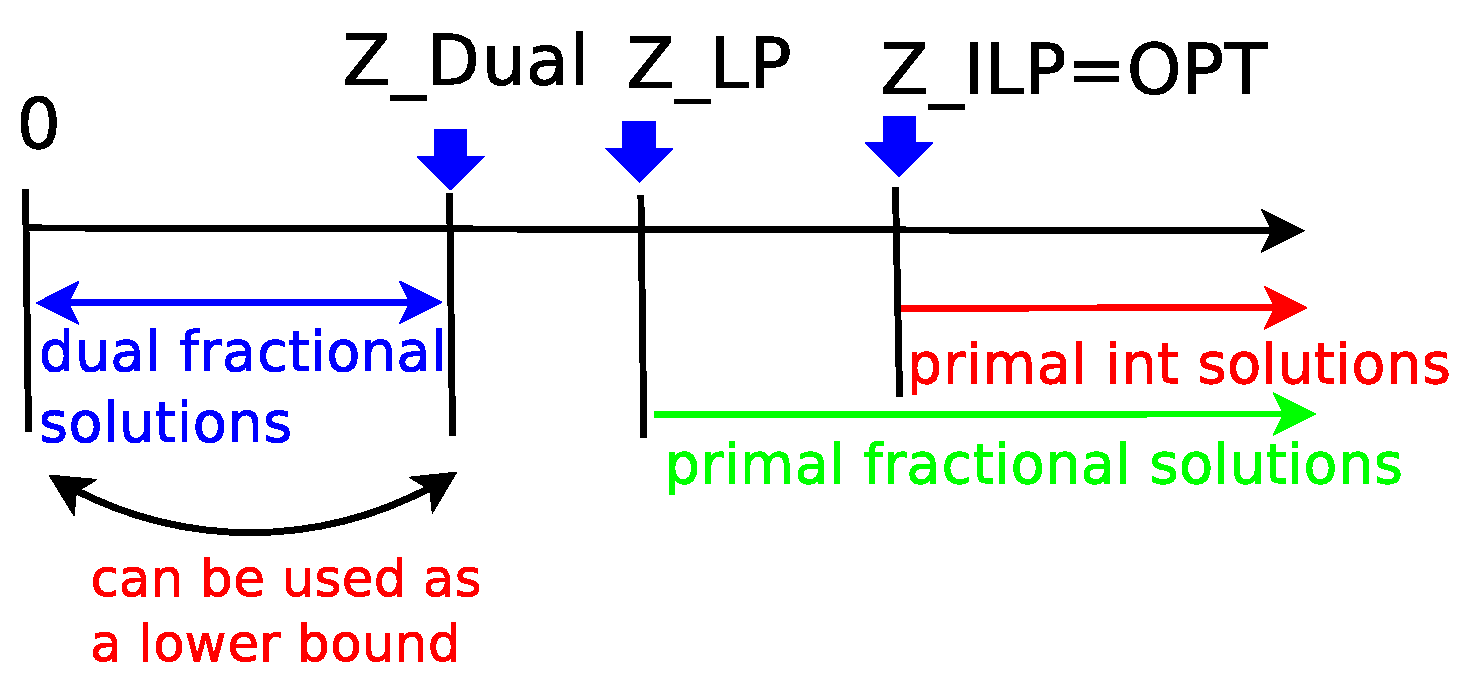
\includegraphics[width=2.5in]{L11-LPlowerbounding.eps}
\end{figure}
} 

\frame{
\frametitle{Algorithm3: Primal\_dual + Rounding } 

Primal\_Dual + Rounding Algorithm3\\
\begin{algorithmic}[1]
\STATE $I=\texttt{NULL}$;
\STATE $y_e = 0$ for all $e \in U $;\
\WHILE{exists an element $\hat{e}$ not covered }
\FORALL{ subset $S_j$ containing $\hat{e}$}
\STATE $g_j = w_j - \sum_{e: e \in S_j} y_e$; // calculate the gap of constraint $j$;
\ENDFOR
\STATE $i = \arg \min_j g_j$; 
\STATE $y_{\hat{e} } = y_{\hat{e} } + g_i$;
\STATE $I = I \cup \{i\}; $
\ENDWHILE
\RETURN $I$;
\end{algorithmic}

% \begin{figure}
%  \includegraphics[width=1.5in]{L11-setcoveralgorithm3.eps}
%  % setcover1.eps: 22002048x0 pixel, 300 dpi, 186284.00x0.00 cm, bb=14 14 407 318
% \end{figure}
}

\frame{
\frametitle{ An example: Step 1 }

\begin{figure}
 \includegraphics[width=1.8in]{L11-setcoverexampledualstep1.eps}
\end{figure}

\begin{itemize} 
\item 
Initially, we have $y_i = 0$ for all $1 \leq i \leq 8$. 
\item 
Consider element $y_2$. There are two constraints $S_1$ and $S_4$. 
\item 
We increase $y_2$ to 3 (selecting $S_4$).
\end{itemize} 
} 

\frame{
\frametitle{ An example: Step 2 }

\begin{figure}
 \includegraphics[width=1.8in]{L11-setcoverexampledualstep2.eps}
\end{figure}

\begin{itemize} 
\item 
Consider element $y_1$. There are two constraints $S_1$ and $S_3$. 
\item 
We increase $y_1$ to 3 (selecting $S_1$).
\end{itemize} 
} 

\frame{
\frametitle{ An example: Step 3 }

\begin{figure}
 \includegraphics[width=1.8in]{L11-setcoverexampledualstep3.eps}
\end{figure}
\begin{itemize} 
\item 
Consider element $y_7$. There are three constraints $S_2$, $S_3$ and $S_5$. 
\item 
We increase $y_7$ to 2 (selecting $S_2$).
\end{itemize} 
} 

\frame{
\frametitle{ An example: Step 4 }

\begin{figure}
 \includegraphics[width=1.8in]{L11-setcoverexampledualstep4.eps}
\end{figure}
\begin{itemize} 
\item 
All elements have been covered. Done! 
\item 
Dual solution: $y_1 = 3; y_2 = 3; y_7 = 2; y_3 = y_4 = y_5 = y_6 = y_8 = 0;$. 
\item 
Dual objective  value:  8.  (Dual feasible solution, $z \leq z_{Dual} \leq z_{LP} \leq z_{ILP} = OPT $) 
\item 
Tight constraints: $I=\{ S_4, S_1, S_2\}$
\item 
Objective  value: $11 \leq d \times z \leq d \times z_{Dual} \leq d \times OPT$
\end{itemize} 
}




\frame{
\frametitle{Correctness}
\begin{small}
\begin{lemma}
 Algorithm3 yields a dual feasible solution $y$, and $\sum_{e: e \in S_j} y_e=w_j$ for any $j \in I$. 
\end{lemma}
\begin{Proof}
\begin{itemize}
\item Base case:  $y=0$ is dual feasible since $\sum\nolimits_{e: e \in S_j} y_e = 0 \leq w_j$; 
 \item Induction: assuming that $y$ is dual feasible before an iteration of while loop, i.e.  $\sum_{e: e\in S_j} y_e  \leq w_j$.  Suppose we increase $y_{\hat{e}}$ by $g_i$ to generate a new solution $y'$. We will show that $y'$ is also a dual feasible solution.  
 \begin{eqnarray}
 \sum\nolimits_{e: e\in S_j} \hat{y'_e} &=&   \sum\nolimits_{e: e \in S_j} y_e + g_i \text{\quad ($g_i$ is minimal)}\nonumber \\ 
 &=& \sum\nolimits_{e: e\in S_j} y_e + ( w_i - \sum\nolimits_{e: e\in S_i} y_e ) \nonumber \\
 &\leq& \sum\nolimits_{e: e \in S_j} y_e + ( w_j - \sum\nolimits_{e: e\in S_j} y_e ) \nonumber \\ 
 &=& w_j \nonumber 
 \end{eqnarray}
\end{itemize}
\end{Proof}
\end{small}
}

\frame{
\frametitle{Performance analysis }
\begin{Theorem}
 (Bar-Yehuda, Even '81) Algorithm3 is a $d$-approximation algorithm. 
\end{Theorem}
\begin{Proof}
 Let $C$ denote the sum weight of subsets generated by Algorithm2, i.e.  $C=\sum_{j \in I} w_j$. We have:
 \begin{eqnarray}
  C &=& \sum\nolimits_{j \in I} w_j \nonumber \\ 
    &=& \sum\nolimits_{j \in I} \sum\nolimits_{e: e\in S_j} y_e \quad \text{( by lines 9-10) } \nonumber \\ 
    &\leq& d \sum\nolimits_{e: e\in U } y_e \quad \text{( e is covered at most f times) } \nonumber \\ 
    & \leq  & d z_{Dual} \nonumber  \quad ( y \text{ is a dual feasible solution } ) \nonumber \\
    &\leq& d OPT \quad \text{(since y is only a dual feasible solution)} \nonumber
 \end{eqnarray}
\end{Proof}

% Note: the last one is $\leq$ since $y$ is only a feasible solution rather than an optimal solution as in Algorithm2.
}

\frame{
\begin{block}{}
Another example of rounding: the generalization of {\sc Makespan} problem
\end{block}
}

\frame{
\frametitle{ The generalization of {\sc Makespan} problem }

Practical problem: We have multiple servers to process a set of jobs. \textcolor{red}{However, some machines cannot be assigned to a job}. How to schedule jobs to machines as ``balanced'' as possible? 

\begin{figure}
 \includegraphics[width=1.5in]{L11-makespanLPalgoinput.eps}
\end{figure} 
} 

\frame{
\frametitle{Formulation} 

\begin{block}{}
 {\bf INPUT: }  \\ 
$m$ servers $M_1, M_2, ..., M_m$, $n$ jobs $J=\{1,..,n\}$ (each job $j$ has a processing time $t_j$). \textcolor{red}{Each job $j$ has a subset of machines $S_j \subset \{M_1, ..., M_m\}$  that it can use.}

 {\bf OUTPUT: } \\ 
An assignment of jobs to machines to minimize the {\it makespan }, i.e.  the maximum load on any machine, $T=\max_i \sum\nolimits_{j\in A(i)} t_j$, where $A(i)$ denotes the jobs assigned to machine $i$; 
\end{block}
}

\frame{
\frametitle{ ILP formulation}

(ILP) 
\[
\begin{array}{rrrrrrrrl}
 \min & L  \\
 s.t. & \sum_{i=1}^m x_{ji} &=& t_j  & \text{for all  }  j \in J \\ 
      & \sum_{j=1}^n x_{ji} &\leq& L & \text{for all }  i \\
      &\textcolor{red}{ x_{ji} }&\textcolor{red}{=}& \textcolor{red}{0/t_j}             & \text{for all  }  j \in J, i \in S_j \\
      & x_{ji} &=& 0                 & \text{for all  }  j \in J, i \notin S_j \\
\end{array} \nonumber
\]

(Intuition: $x_{ji}$ indicates  how much of the load of $t_j$ is assigned to machine $M_i$; )

} 


\frame{
\frametitle{ Relax from ILP to  LP }

(LP) 
\[
\begin{array}{rrrrrrrrl}
 \min & L  \\
 s.t. & \sum_{i=1}^m x_{ji} &=& t_j  & \text{for all  }  j \in J \\ 
      & \sum_{j=1}^n x_{ji} &\leq& L & \text{for all }  i \\
      &\textcolor{red}{ x_{ji} }&\textcolor{red}{\leq}& \textcolor{red}{t_j}             & \text{for all  }  j \in J, i \in S_j \\
      &\textcolor{red}{ x_{ji} }&\textcolor{red}{\geq}& \textcolor{red}{0}             & \text{for all  }  j \in J, i \in S_j \\
      & x_{ji} &=& 0                 & \text{for all  }  j \in J, i \notin S_j \\
\end{array} \nonumber
\]

\begin{itemize}
 \item 
\textbf{Key observation 1:} $z_{LP} \leq z_{ILP} = OPT$ \\
\item
\textbf{Key observation 2:} $\max_j t_j \leq OPT$ \\ 
\end{itemize}
} 

\frame{
\frametitle{ An example }

\begin{figure}
 \includegraphics[width=1.5in]{L11-makespanLPalgoinput.eps}
\end{figure}

(LP) 
\[
\begin{array}{rrrrrrrrl}
 \min z=& L  \\
 s.t. &           &  x_{12}  & +x_{13}   &=& 6 \\
      & x_{21} & + x_{22} & +x_{23}    &=& 9 \\
      & x_{31} & + x_{32} & +x_{33}    &=& 15 \\
      &            &  x_{21} & +x_{31}     &\leq& L \\ 
      &   x_{12}   & +  x_{22} & +x_{32}     &\leq& L \\ 
      &   x_{13}   & +  x_{23} & +x_{33}     &\leq& L \\ 
      &                &                &   x_{ji}     & \geq & 0 \\
\end{array} \nonumber
\]
}

\frame{
\frametitle{ How to construct a valid schedule from LP solution? }

\begin{figure}
 \includegraphics[width=1.4in]{L11-makespanLPalgosolution.eps}
\end{figure}
\begin{itemize}
 \item Suppose we have already obtained a solution to the LP. The final question is: how to construct a valid schedule from the LP solution? 
 \end{itemize} 
} 


\frame{
\frametitle{ How to construct a valid schedule from LP solution? }
\begin{figure}
 \includegraphics[width=1.4in]{L11-makespanLPalgosolution.eps}
\end{figure}
 
 \begin{itemize} 
 \item Recall that for any job $j$, we have $t_j = x_{j1} + x_{j2} + ...+x_{jm}$. There are two possible cases: 
 \begin{enumerate}
  \item $\exists i, x_{ji} = t_j$ (called ``integral job''): Intuitively, job $j$ was scheduled to machine $M_i$ as a whole, e.g. job $1$. 
  \item $\forall i, x_{ji} < t_j$ (called ``fractional job''): Intuitively, job $j$ was decomposed into parts, which were distributed to different machines, e.g., two parts of job $2$ was distributed to $M_1$ and $M_2$. 
  \end{enumerate}
  \item The difficulty is  how to deal with fractional jobs. 
 \end{itemize} 
 }

\frame{
\frametitle{Two possibilities of the fractional jobs} 
\begin{figure}
 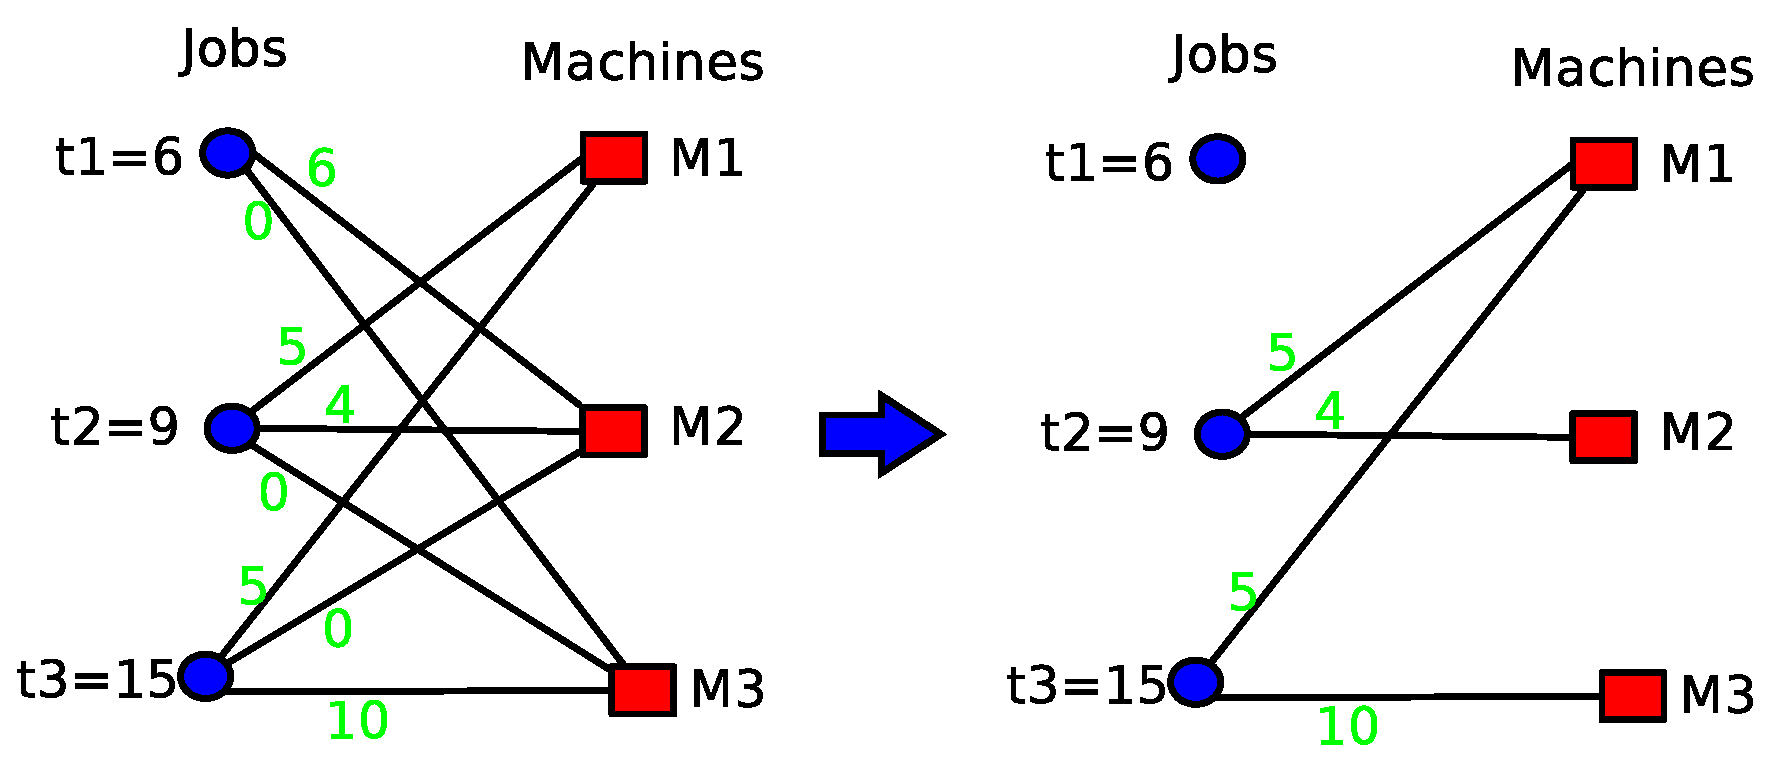
\includegraphics[width=3in]{L11-makespanLPalgosolutionfractionaljobs.eps}
\end{figure}
\begin{itemize} 
\item 
Let's focus on the fractional jobs via: 
\begin{itemize}
\item Removing the "integer jobs"; 
\item Removing the \textbf{unused assignments}, i.e. $x_{ji}=0$; 
\end{itemize}
\item There are two possibilities: 
\begin{enumerate}
	\item The assignment contains \textcolor{red}{ no cycle}; 
	\item The assignment contains \textcolor{red}{one or more cycles};
\end{enumerate}

\end{itemize}
}

\frame{
\frametitle{ Case 1:  the assignment contains no cycle }
\begin{itemize}
\item In this case, a valid schedule can be constructed via the following rounding strategy: 
 \begin{enumerate}
  \item Rounding: If a part of a  fractional job $j$ was scheduled to machine $M_i$, we can simply schedule the whole job $j$ to $M_i$. 
  \item Restriction: Each machine  receives {\bf at most} one fractional job. 
   \end{enumerate}
 \end{itemize}
} 

\frame{
\frametitle{ Implementing rounding }

   \begin{figure}
 \includegraphics[width=4in]{L11-makespanLPalgosolutionfractionaljobstree.eps}
\end{figure}
\begin{itemize}
\item The rounding operation is feasible since: 
\begin{enumerate}
	\item ``No cycle" means a tree rooted at a job. 
	\item Notice that any leaf should be a ``machine" rather than a ``job" (Reason: a ``leaf job" is connected with its parent only; thus it should be an ``integer job")
	\item So we can simply assign a fractional job {\bf completely}  to an {\bf arbitrary} child, say assign $J_2$ to $M_1$, and assign $J_3$ to $M_2$.
\end{enumerate}
\item Time complexity: $O(mn)$.
 \end{itemize}
} 



\frame{
\frametitle{ Case 1:  the assignment contains no cycle  cont'd}
\begin{itemize}
\item Combining the "integer jobs", we will have the following schedule: 
 \item $J_{M1}=\{ 2\}; J_{M2}=\{1\}; J_{M3}=\{3\}$. 
 \begin{figure}
 \includegraphics[width=3in]{L11-makespanLPalgosolutioncase1.eps}
\end{figure}
 \item MakeSpan= $15 \leq 2\times z_{LP} = 20$
 \item We can show that the rounding strategy won't introduce too many load to any machine. 
 \end{itemize}


}

\frame{
\frametitle{}
\begin{Theorem}
$MakeSpanApprox$ is a $2$-approximation algorithm.  
\end{Theorem}
\begin{Proof}
\begin{footnotesize}
 
\begin{itemize}
 \item Let $T$ denotes the makespan that $MakeSpanApprox$ yields, and $T$ is obtained from machine $M_i$. 
 \item Let $J_i$ denote the jobs assigned to $M_i$.  $J_i$ consists of two parts: integral jobs assigned to machine $i$ ($x_{ij} = t_j$), and at most \textcolor{red}{\bf one} fractional job (denoted as $f_i$) that is assigned to multiple machines ($x_{ij} < t_j$). We have: 
%  \item Removing cycle: increasing flow on a cycle by the smallest capacity $\delta$ in the residual graph. Thus, an edge of the cycle will be removed, and a ``bad'' job changes to a ``good'' job. 
\end{itemize}
 \begin{eqnarray} 
   T & = & \sum\nolimits_{j\in J_i } t_j \\
     & = & \sum\nolimits_{j\in J_i, j\neq f_i } t_j + t_{f_i} \\ 
     & = & \sum\nolimits_{j\in J_i, j\neq f_i } x_{ij} +  t_{f_i} \quad \text{ (by the definition of integral jobs)}\\
     & \leq & \sum\nolimits_{j\in J_i  } x_{ij} +  t_{f_i}  \\ 
     & \leq & z_{LP}  +  t_{f_i}  \\
     & \leq & z_{LP}  +  OPT  \quad \text{( by key observation 2) } \\
     & \leq & 2 OPT  \quad \text{(by key observation 1)}
  \end{eqnarray}
\end{footnotesize}
\end{Proof}
} 


\frame{
\frametitle{ Case 2: the assignment contains cycles } 
\begin{itemize}
 \item In fact, any cycle can be eliminated  without load changes for any machine using the following 
 \textcolor{red}{\bf ``augmentation"} operation: 
\begin{enumerate}
  \item Consider a cycle $C$.  We first find the smallest load (denoted as $\delta$); 
 \item Increasing/decreasing loads  by $\delta$ on edges in the cycle; 
 \item Thus the cycle will be eliminated without  no influence on the loads. For example, edge $J_1-M_3$ is cut to break the cycle.  
 \end{enumerate}
 \item Time complexity: $O(|C|)$ for cycle $C$. The operation will be repeated at most $O(mn)$ times to remove all cycles. 
\begin{figure}
 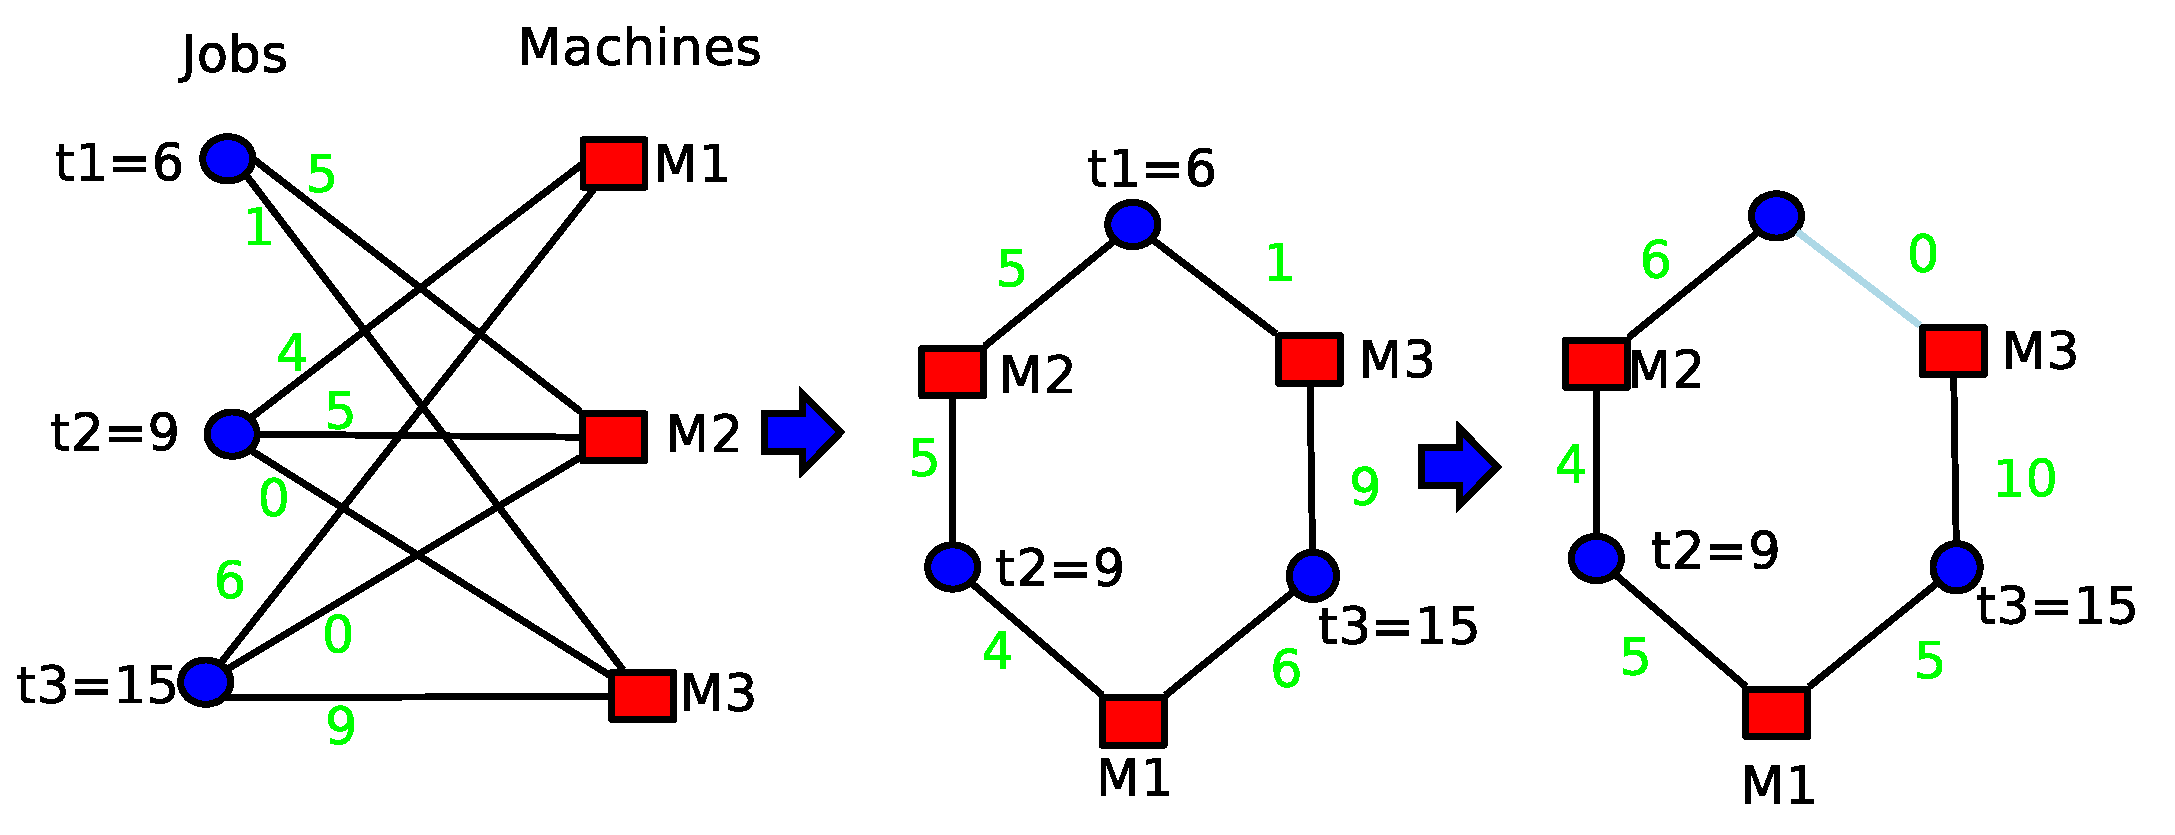
\includegraphics[width=3.8in]{L11-makespanLPalgosolutioncase2tree.eps}
\end{figure}
\end{itemize}
} 

\frame{
\frametitle{ }

{\sc MakeSpanApprox} Algorithm
\begin{algorithmic}[1]
\STATE Solving the LP model to get solution $x_{ij}$; 
\STATE Removing cycles in the schedule graph via \textcolor{red}{\bf augmentation}; 
\FOR{ $i=1$ to $m$ } 
\STATE assigning integral job $j$ to $i$ if $x_{ij} = t_j$; 
\STATE assigning at most \textcolor{red}{\bf one} fractional  job to $i$; 
%\STATE removing job $j$ and machine $i$; 
\ENDFOR
\end{algorithmic}


}


\frame{
\begin{block}{} 
Other useful technique: scaling and parametric pruning 
\end{block} 
} 

\frame{
\frametitle{ Other combinatorial techniques}
\begin{block}{}
\begin{itemize}
\item 
Scaling: rounding a real number to an integer; grid;  \\
\item 
Parametric pruning: Suppose we have already known $OPT$, we might be able to prune away irrelevant parts of the input and thereby simplify the search for a good solution. 
\end{itemize}
\end{block}
}

\frame{
\begin{block}{}
 Scaling technique:  from pseudo polynomial time algorithm to PTAS
\end{block}
}

\frame{
\frametitle{ {\sc Knapsack} problem}
Given a set of items, each item has a weight and a value, to determine a set of items such that the total weight is less than a given limit and the total value is as large as possible.
\begin{block}{Formalized Definition:}
\begin{itemize}
    \item {\bf Input:}\\ a set of items. Item $i$ has weight $w_i$ and value $v_i$, and a total weight limit $W$; 
	\item {\bf Output:}\\ the set of items which maximize the total value with total weight below $W$
\end{itemize}
 %\begin{itemize}
 %\item {\bf Input:} \\a set of items $i$ with weight $w$_$i$ and value $v$_$i$, and a total weight limit $W$, $i$=1,2,\cdots,$n$
 %\item {\bf Output:}\\the set of items which maximize the total value with total weight below $W$
 %\end{itemize}
\end{block}
}

\frame
{
	\frametitle{A Knapsack instance}
	\begin{center}
	What's the best solution?
	\end{center}
	\begin{figure}
	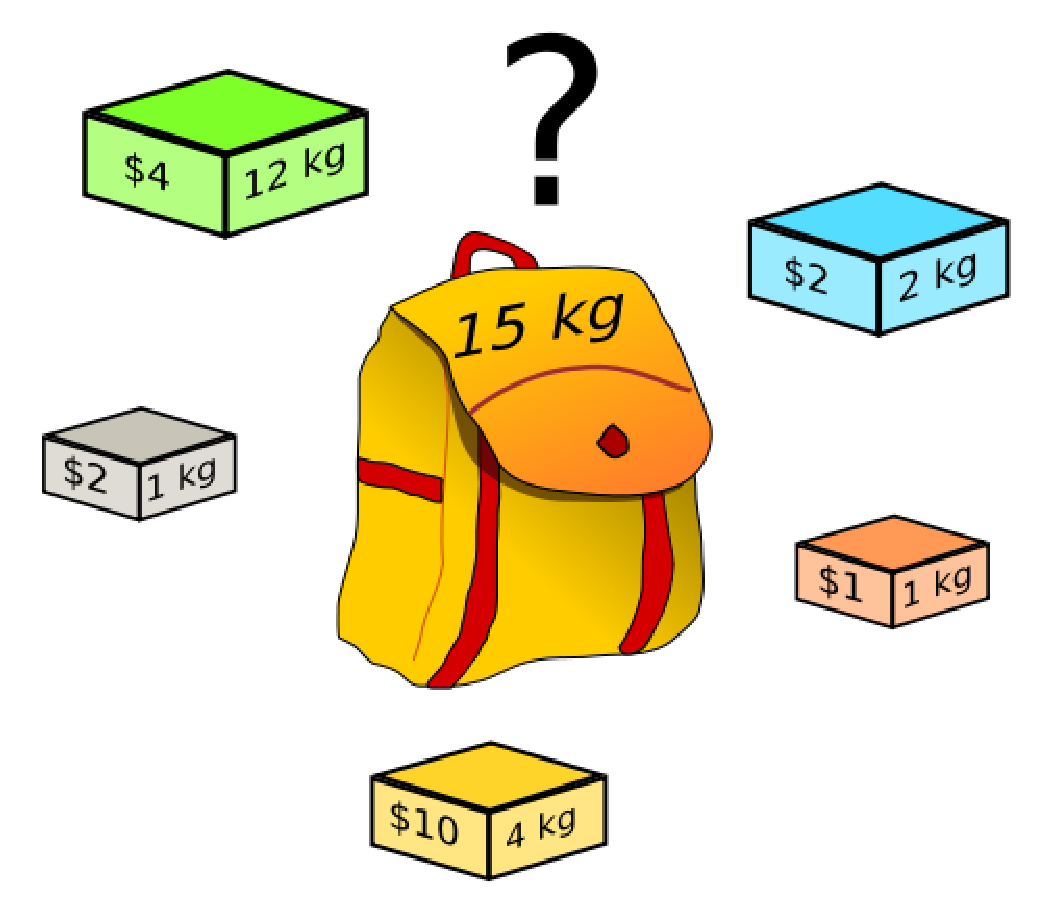
\includegraphics[width=2in]{486px-Knapsack.eps}
	\end{figure}
}

\frame{
\frametitle{A Knapsack instance}
	\begin{center}
	Greedy solution:
	\end{center}
	\begin{figure}
	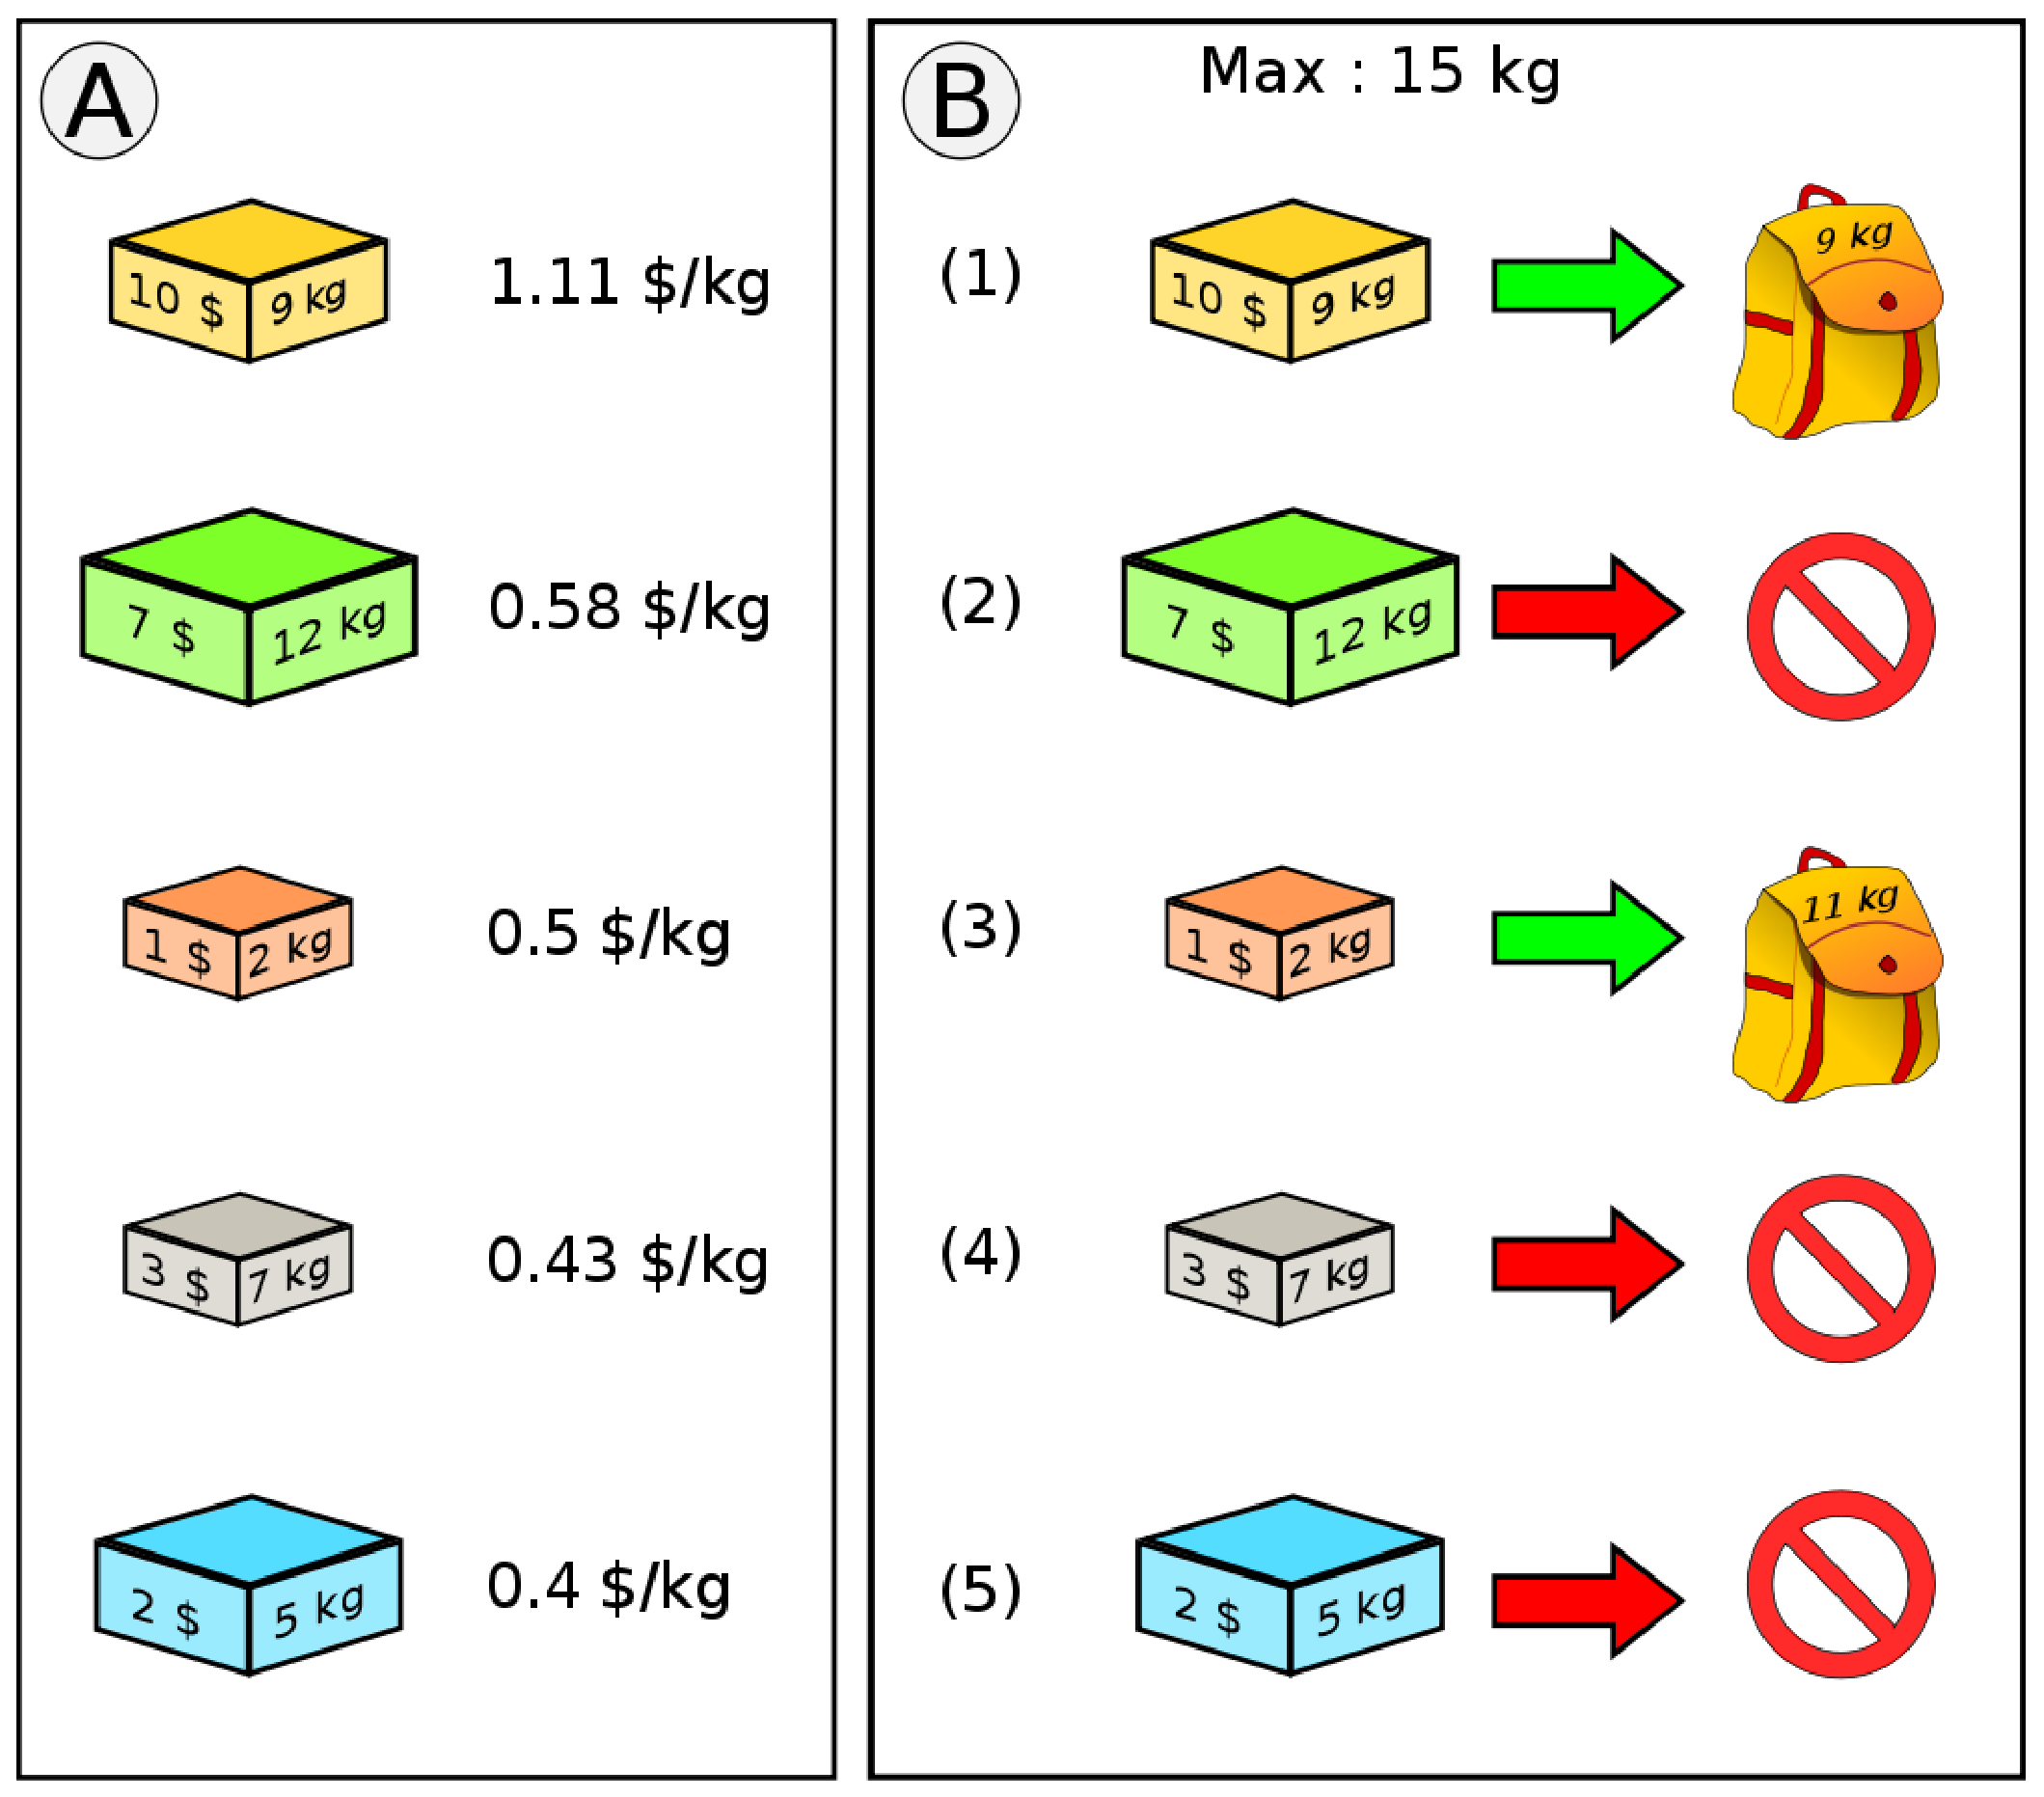
\includegraphics[width=2.3in]{1000px-Knapsack_greedy.eps}
	\end{figure}
	
Note: there are two types of dynamic programming algorithms to solve {\sc Knapsack} problem. 
}

\frame{
\frametitle{ Dynamic programing algorithm 1 } 

\begin{itemize}
 \item Imagine the solving process as a series of decisions. 
%  \item At each step, we make a decision that whether item $k$ should be selected or abandoned. 
\item Suppose we have already obtained the optimal solution $S$. Let's consider the first decision step, we have two options: select item $n$, or abandon it. 
\item Thus the general form of sub-problems can be set as: to calculate the maximum value of any solution using a subset of the items $\{1,2,...,i\}$ and a bag of size $w$, denoted as $OPT(i, w)$. \\
\item 
Our objective: $OPT( n, W)$. 
\item 
Optimal sub-structure: 
$OPT( n, W ) = max\{ OPT(n-1, W), OPT(n-1, W-w_n) + v_n \}$;
\end{itemize}

	\begin{figure}
	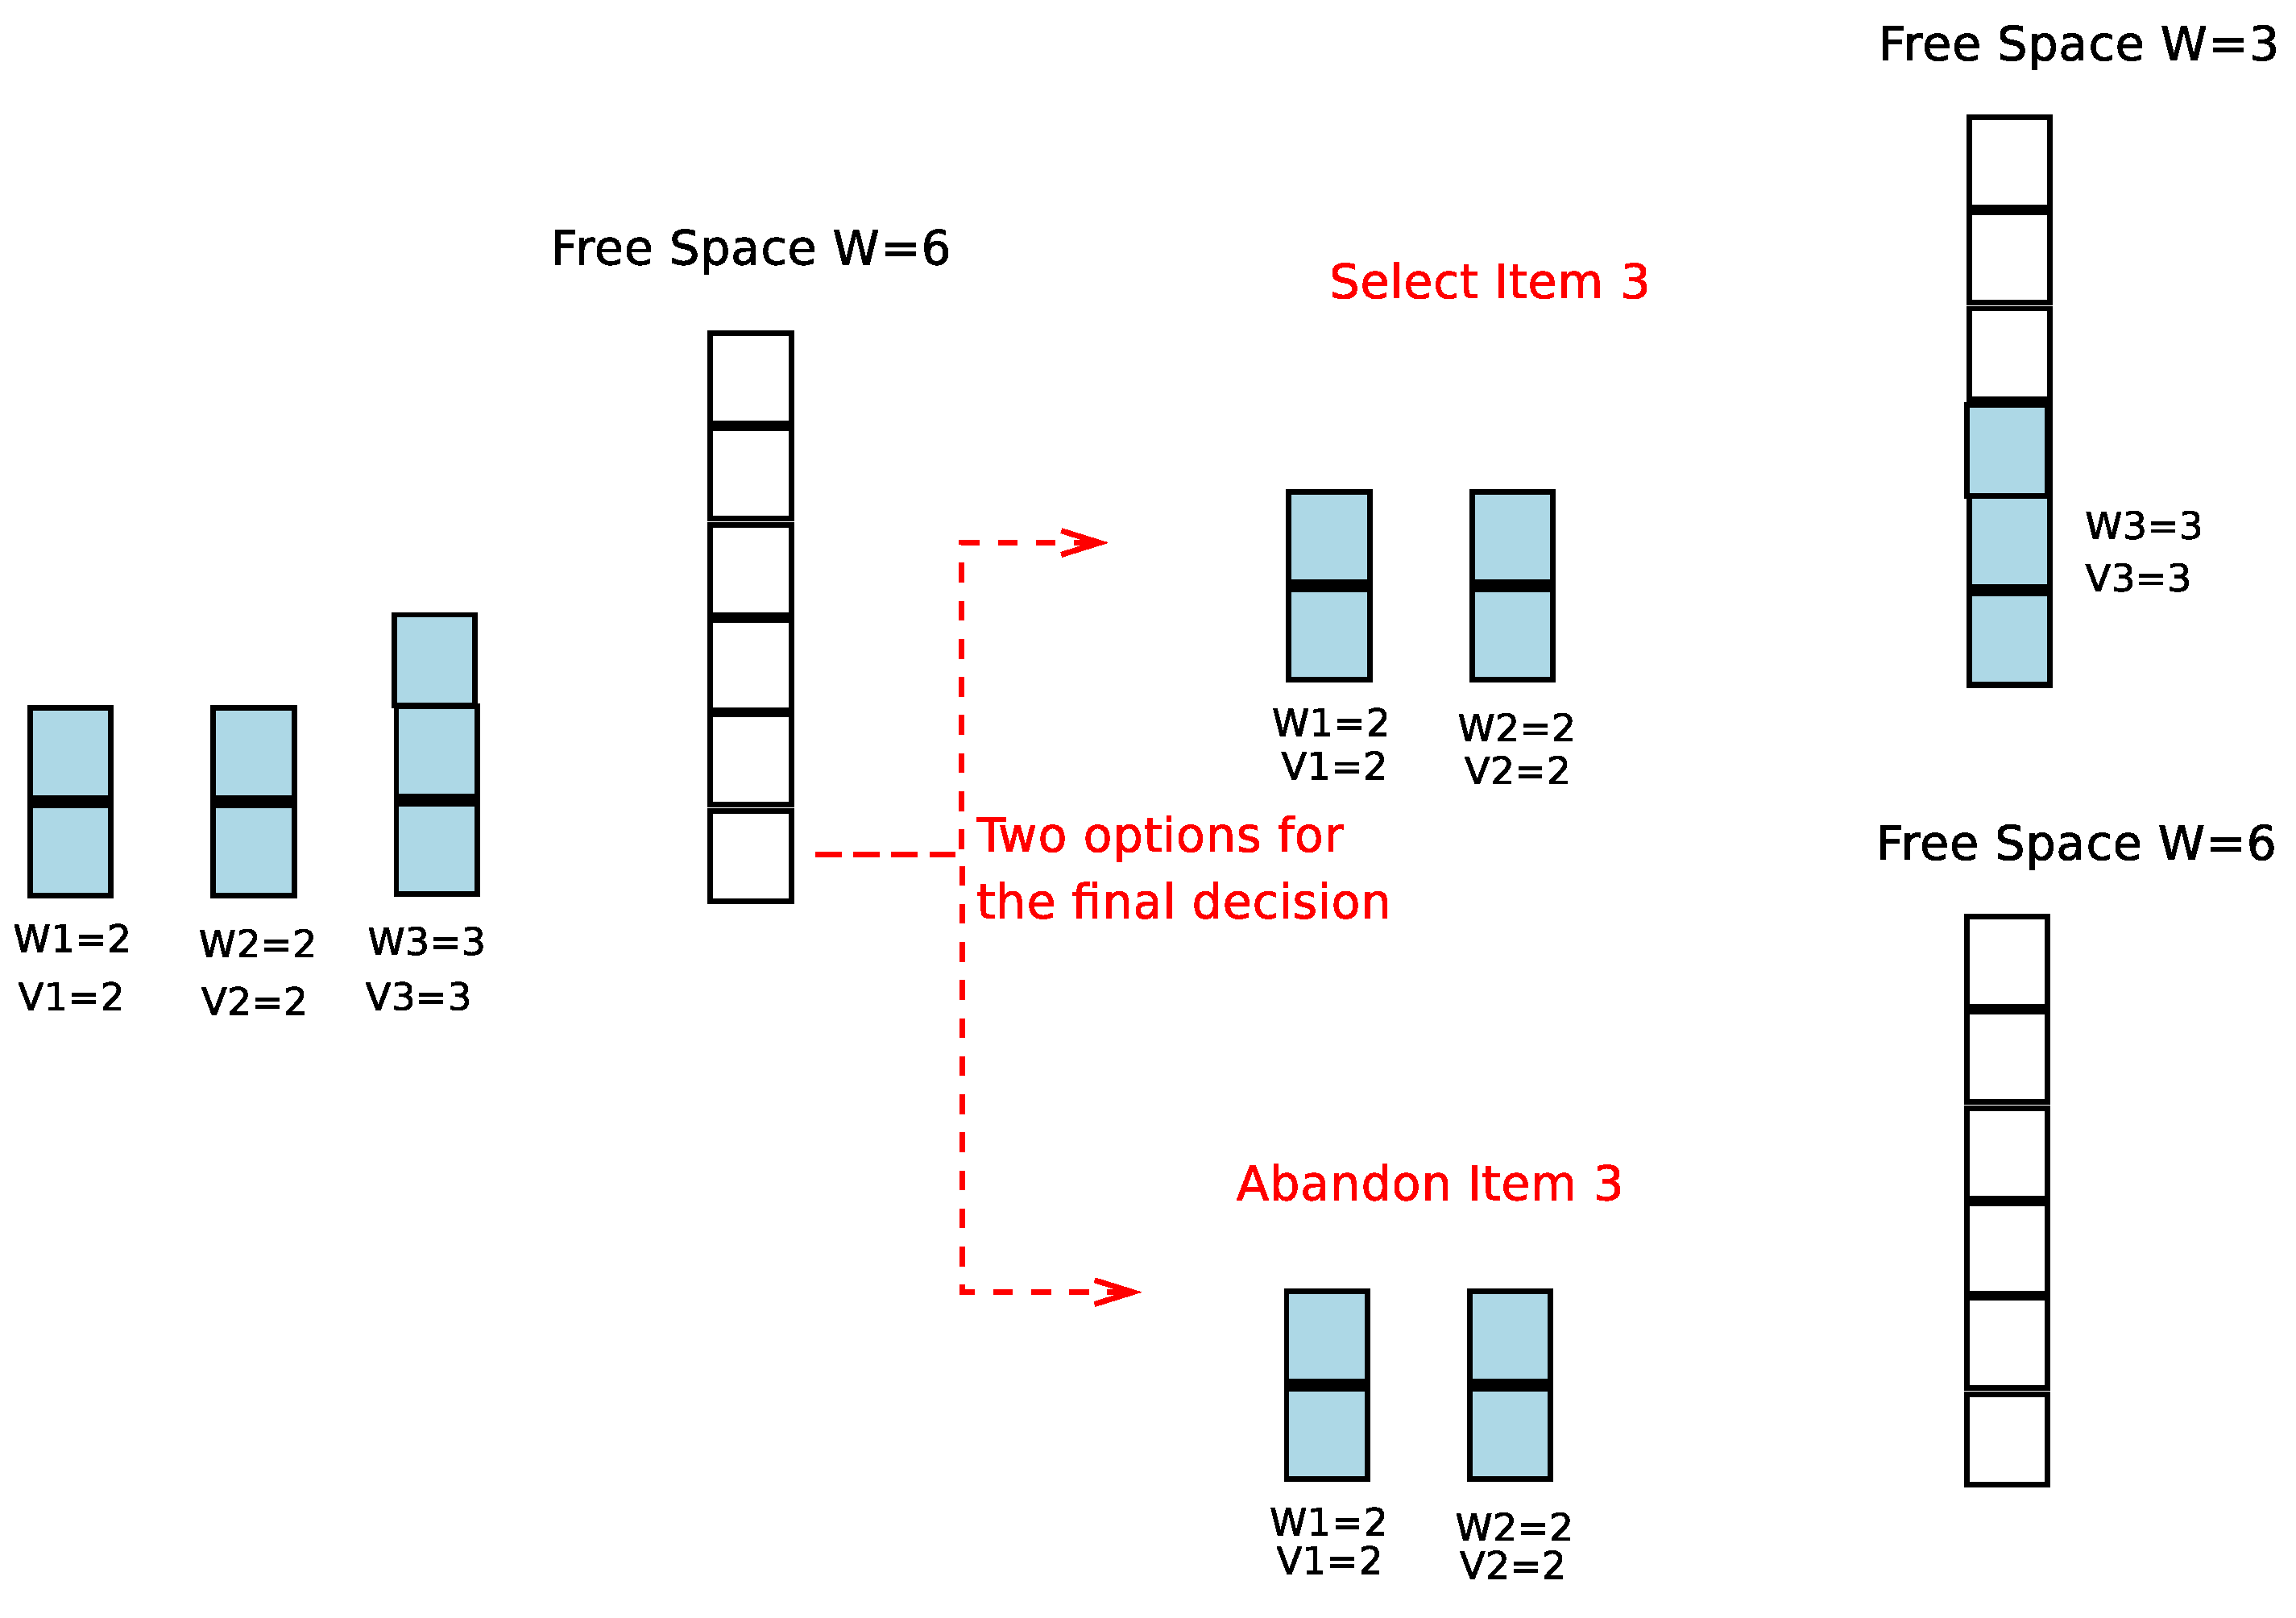
\includegraphics[width=2.5in]{L6-Knapsackexample.eps}
	\end{figure}

}

\frame{
\frametitle{}

Knapsack DP1\\
\begin{algorithmic}[1]
\FOR {$w=1$ to $W$} 
\STATE $M[0,w] = 0$;
\ENDFOR

\FOR {$i=1$ to $n$}
\FOR {$w=1$ to $W$} 
\STATE $M[i,w] = max\{M[i-1,w],w_i + M[i-1,w-w_i]\}$;
\ENDFOR
\ENDFOR
\RETURN $M[n,W]$;
\end{algorithmic}


% 	\begin{figure}
% 	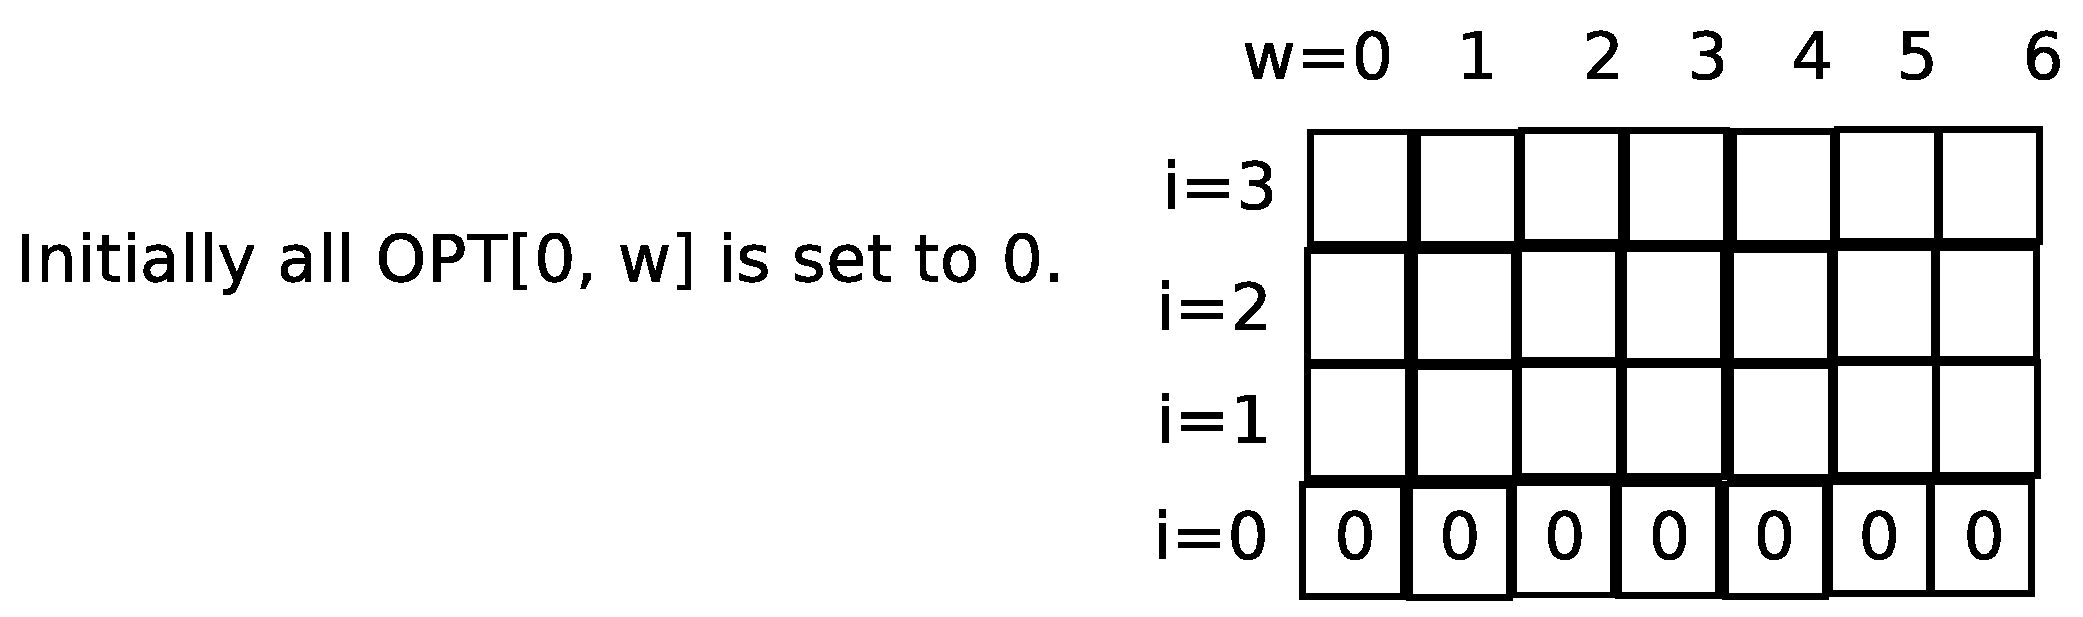
\includegraphics[width=4in]{L6-Knapsackalgostep1.eps}
% 	\end{figure}
% 	\begin{figure}
% 	\includegraphics[width=4in]{L6-Knapsackalgostep2.eps}
% 	\end{figure}	
% 	\begin{figure}
% 	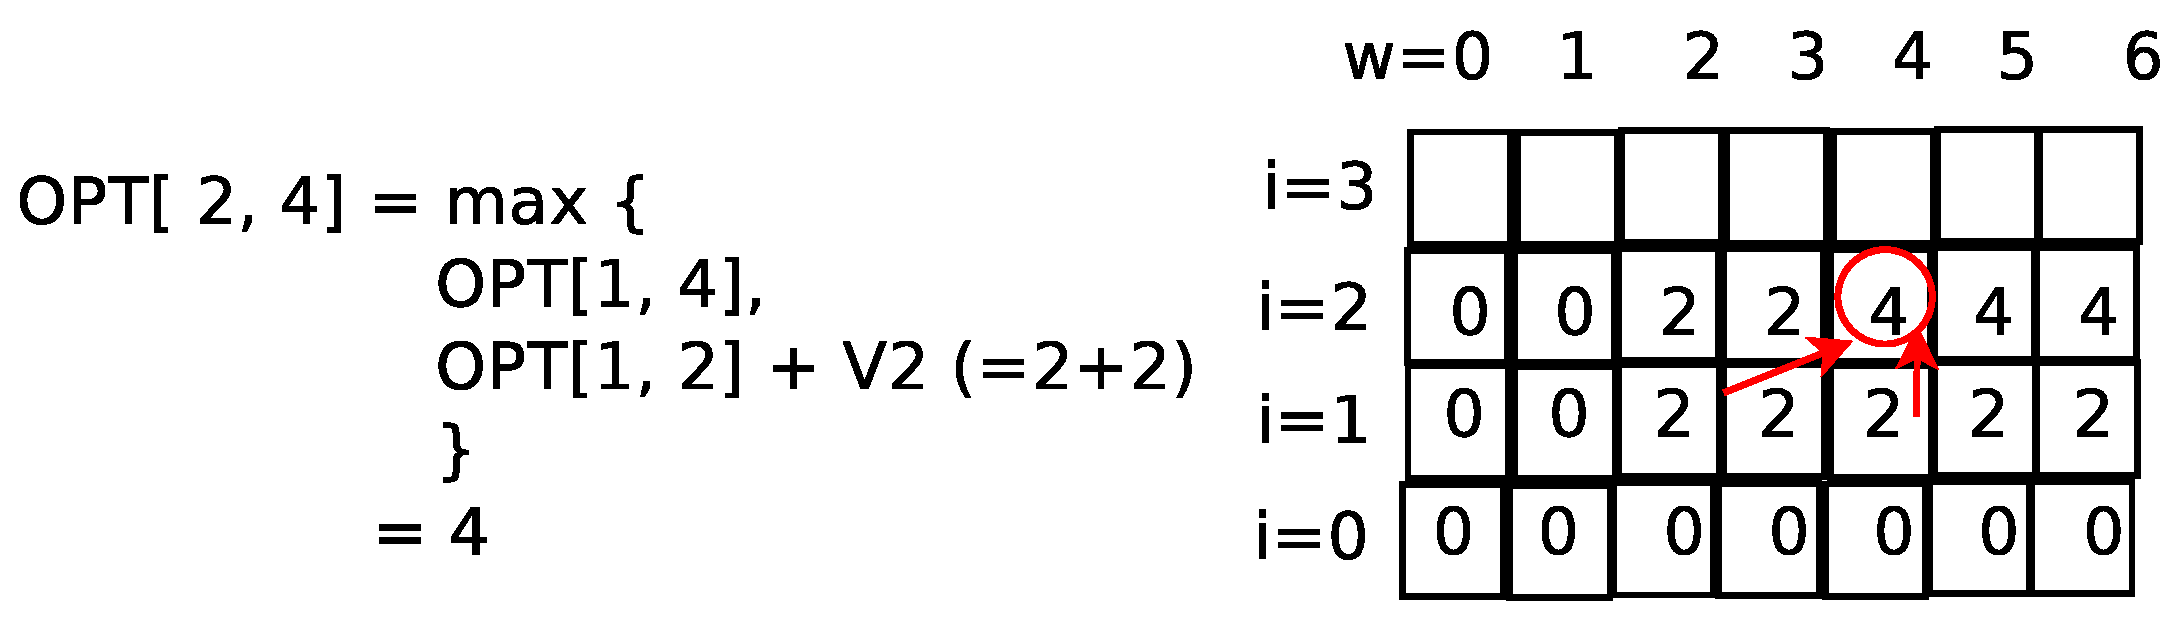
\includegraphics[width=4in]{L6-Knapsackalgostep3.eps}
% 	\end{figure}	
% 	\begin{figure}
% 	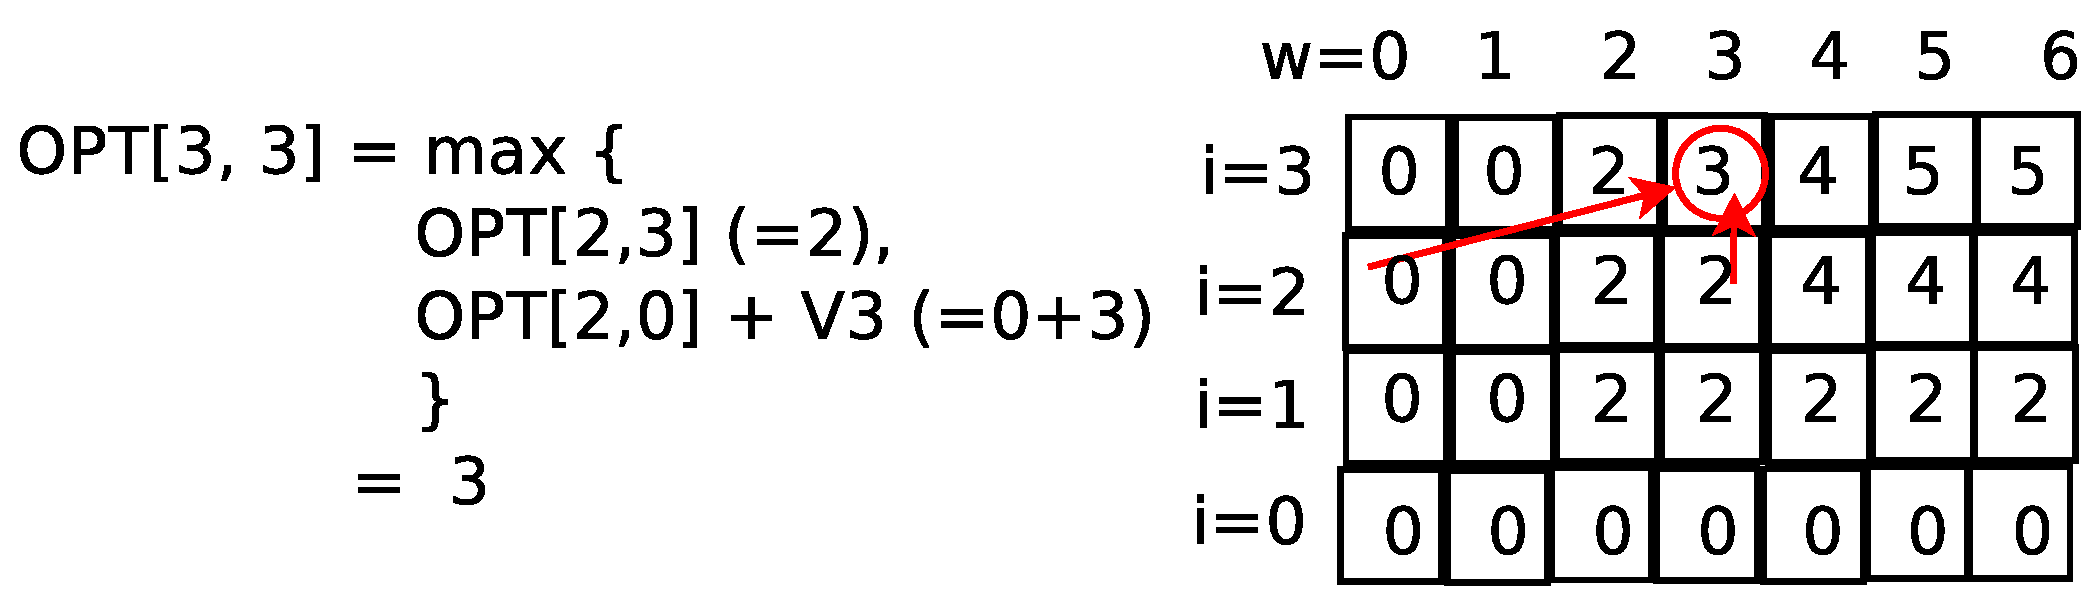
\includegraphics[width=4in]{L6-Knapsackalgostep4.eps}
% 	\end{figure}

Time complexity: $O(nW)$. Pseudo polynomial time.
} 

%\frame{
%\frametitle{A tightly related problem}
%
%\begin{itemize}
%    \item {\bf Input:}\\ a set of items. Item $i$ has weight $w_i$ and value $v_i$, and a value requirement $V$; 
%   \item {\bf Output:}\\ the set of items which minimize the total weight with value at least $V$; 
%\end{itemize}
% %\begin{itemize}
% %\item {\bf Input:} \\a set of items $i$ with weight $w$_$i$ and value $v$_$i$, and a total weight limit $W$, $i$=1,2,\cdots,$n$
% %\item {\bf Output:}\\the set of items which maximize the total value with total weight below $W$
% %\end{itemize}
%	
%	\begin{itemize}
%	\item Note: If this problem was solved, the Knapsack problem can be solved by \textcolor{red}{\bf finding the largest value $V$ such that $OPT(n, V) \leq W$. 
%	\end{itemize}
%}


\frame{

\frametitle{ A dual problem} 

\begin{block}{}
{\bf INPUT: } a set of $n$ items. An item $i$ has weight $w_i$ and value $v_i$. The value requirement $V$;
\\

{\bf OUTPUT: } to select a subset of items to minimise the total weight with value at least $V$; 
\end{block} 

Note: if this problem was solved, the Knapsack problem can be solved by by \textcolor{red}{\bf finding the largest value $V$ such that $OPT(n, V) \leq W$.} 
}


\frame{
\frametitle{ Dynamic programming algorithm 2 }


\begin{itemize}
 \item Imagine the solving process as a series of decisions. 
 \item Suppose we have already obtained the optimal solution $S$. Let's consider the first decision step, there are two possibilities: select item $n$ or abandon it; 
 \item The general form of sub-problems: to calculate the smallest bag size, i.e. the bag can hold a subset of items $\{1,2,...,i\}$ with value at least $V$ (denoted as $OPT(i, V)$); \\
\item 
Our objective: the largest $V$ such that $OPT( n, V) \leq W$. (Notice that $V \leq n v^*$, where $v^*=max_i \{ v_i \}$);
\item 
Optimal sub-structure: 

\begin{footnotesize}
$OPT(n, V) = \min\begin{cases}OPT(n-1,V)&\text{abandon item n} \\ 
w_n & \text{select item n only} \\
w_n+OPT(n-1,V-v_n)&\text{otherwise}\end{cases} $
\end{footnotesize} 
\end{itemize}
}

\frame{
\frametitle{ Dynamic programming algorithm 2  cont'd }

Knapsack DP2\\
\begin{algorithmic}[1]
\FOR {$i=0$ to $n$} 
\STATE $M[i,0] = 0$;
\ENDFOR
\FOR {$i=1$ to $n$}
\FOR {$V=1$ to $\sum_{k=1}^{i}v_k$}
\IF{$V > \sum_{k=1}^{i-1}v_k$} 
\STATE $M[i,V] = w_i + M[i-1,V-v_i]$;
\ELSE
\STATE $M[i,V] = min\{M[i-1,V],w_i,w_i + M[n-1,v-v_i]\}$;
\ENDIF
\ENDFOR
\ENDFOR
\end{algorithmic}

%  \begin{figure}
%  	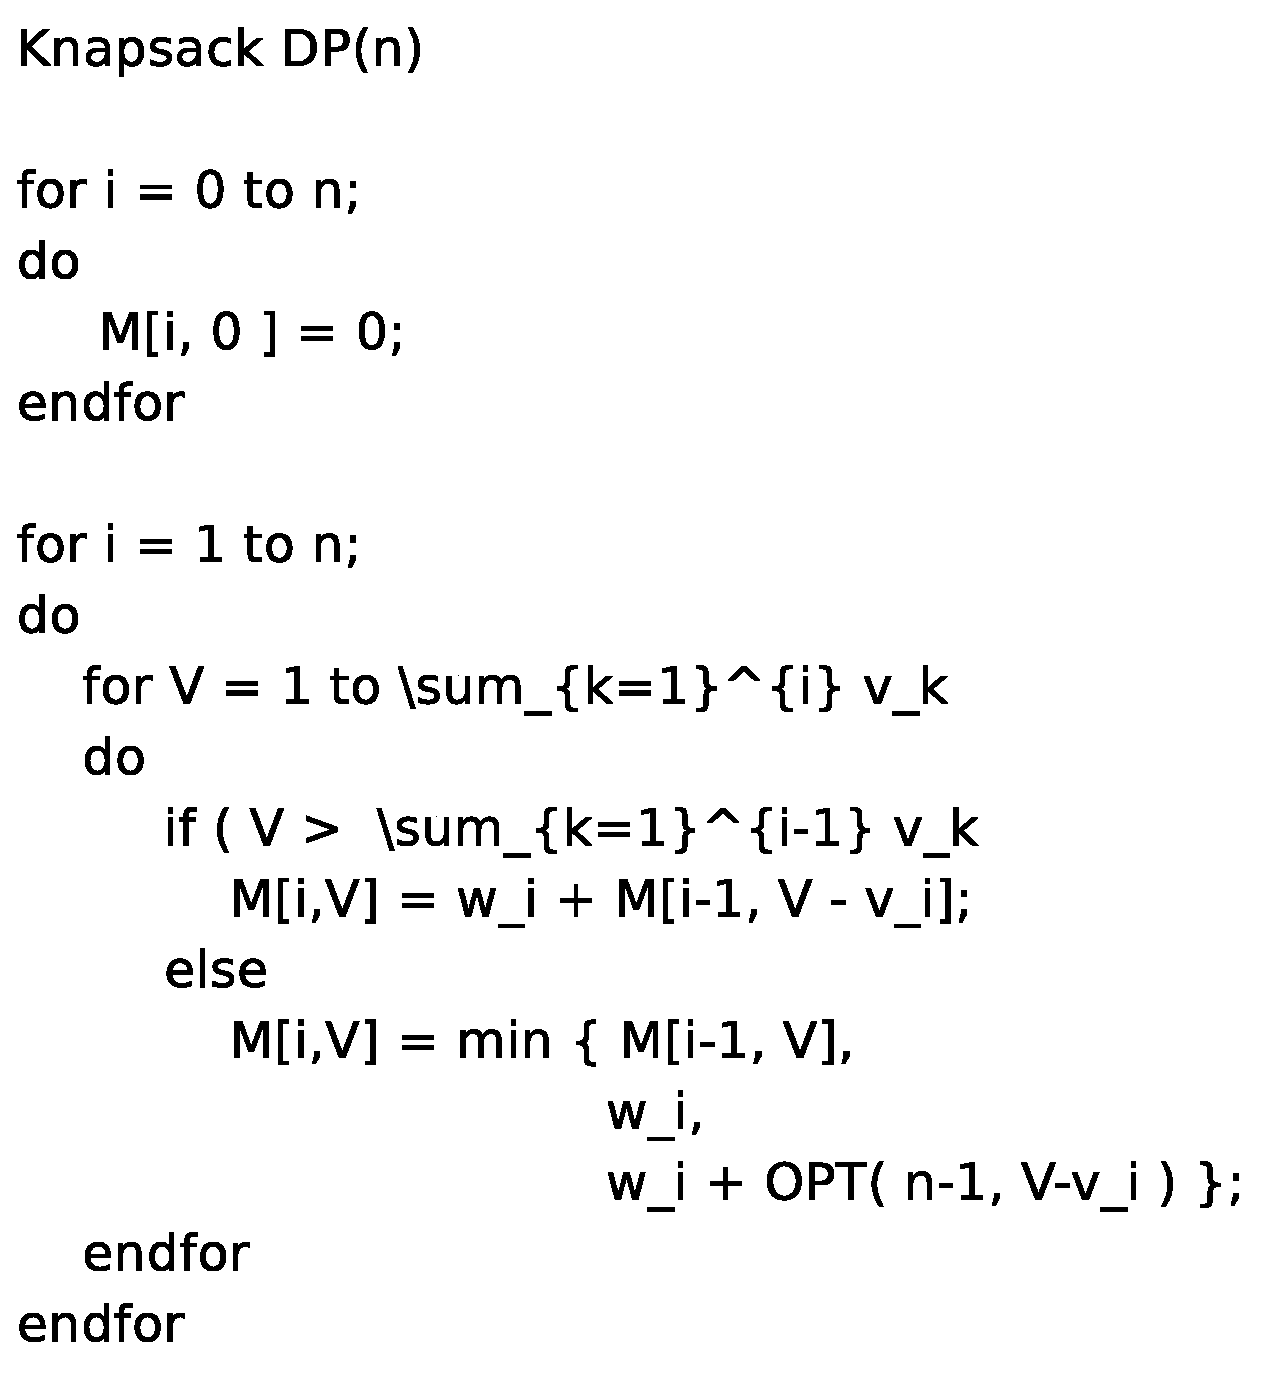
\includegraphics[width=1.5in]{L11-KnapsackDP2.eps}
%  \end{figure} 
Time complexity: $O(n^2 v^*)$. Still pseudo-polynomial time. 
}

\frame{
\frametitle{ Converting pseudo-polynomial time algorithm to PTAS }

\begin{itemize}
 \item 
Basic idea: the algorithm is good when $v^*$ is small. But how to deal with the case when $v^*$ is large? \textcolor{red}{Scaling!}
\item More specifically,  a large $v_i$ can be scaled to a smaller $\hat{v_i} = \lceil \frac{v_i}{b}\rceil$. We denote $\overline{v_i} = \hat{v_i} b$;
\end{itemize}

\begin{figure}
	\includegraphics[width=2.5in]{L11-KnapsackDP2rounding.eps}
\end{figure} 
} 


\frame{
\frametitle{ A PTAS for {\sc Knapsack} }

Knapsack-Approx($\epsilon$) \\
\begin{algorithmic}[1]
\STATE Let $v^* = \max_i v_i$; 
\STATE Let $b= \frac{ \epsilon }{ n } v^*$; 
\STATE Calculate $\hat{v_i} = \lceil \frac{ v_i }{ b } \rceil $ for each item $i$; 
\STATE Run KnapsackDP2 on the items with value $\hat{v_i}$ and return the optimal solution $S$; 
\end{algorithmic}

Knapsack-Approx algorithm runs in polynomial time. 

In fact, the running time is $O(n^2 \hat{v^*}) = O( n^2 \frac{v^*}{  b} ) = O(\frac{n^3}{ \epsilon} )$. 
} 

\frame{
\frametitle{ Experimental results }

Experimental results on an instance: 
\begin{footnotesize}
  \begin{table}
    {\begin{tabular}{r|rrrrrrrr}
    \hline
        $b$ &  $ \overline{v} $&  $\epsilon$ &  $W$ & \# OP & Time (ms) \\
  \hline
         1  &        2223975 &      0.001 &     1768 &  889590000  &      18352.128     \\
         3  &         741325 &        0.010 &     1768 &   98843333  &       5990.893     \\
         5  &         444800 &       0.028 &     1768 &   35584000  &      3649.624     \\
        10  &         222400 &         0.112 &     1768 &    8896000  &       1836.567     \\
        30  &          74125 &          1.011 &     1768 &     988333  &         620.822    \\
        50  &          44475 &         2.810 &     1768 &     355800  &         381.982    \\
       100  &          22250 &          11.236 &    1768  &     89000   &       183.707     \\
       300  &           7425 &          101.010 &     1768 &       9900  &          60.422    \\
       500  &           4450 &         280.899 &     1768 &       3560  &          38.340    \\
      1000  &           2225 &          1123.6 &     1768 &        890  &         17.943     \\
      3000  &            750 &           10000 &     1809 &        100  &           6.872    \\
      5000  &            450 &         27777.8 &     1809 &         36  &          4.059     \\
     10000  &            225 &          111111 &     1809 &          9  &           3.134    \\ \hline
      \end{tabular}} {}%
  \end{table}
\end{footnotesize}
}

\frame{
\frametitle{ Performance analysis  }
\begin{Theorem}
 Let $S$ be the solution yielded by Knapsack-Approx algorithm, and $S^*$ be any feasible solution such that $\sum_{i \in S^*} w_i \leq W$. We will show that  
 $  \sum_{i \in S} v_i  \geq \frac{1}{1+\epsilon}  \sum_{i\in S^*} v_i $. 
\end{Theorem}
\begin{small}
\begin{Proof}
%  Key observation: $\sum_{i\in S^*} v_i \leq \sum_{i\in S^*} \overline{v_i}$. 
  \begin{eqnarray}
   \sum\nolimits_{i\in S^*} v_i &\leq& \sum\nolimits_{i\in S^*} \overline{v_i} \quad \text{ (by } v_i \leq \overline{ v_i}) \\
    &\leq& \sum\nolimits_{i\in S } \overline{v_i} \quad \text{ (S is optimal solution) } \\
    &\leq& \sum\nolimits_{i\in S } ( v_i + b ) \quad \text{ (by } \overline{ v_i} \leq v_i + b)\\
    &\leq& nb + \sum\nolimits_{i\in S }  v_i  \\
    &\leq& (1+\epsilon) \sum\nolimits_{i\in S }  v_i \qquad (\text{since } nb \leq \epsilon \sum\nolimits_{i\in S }  v_i) 
  \end{eqnarray}
\end{Proof}
\end{small}
}

\frame{
\frametitle{ Why $b$ was set to $b=\frac{ \epsilon }{ n } v^*$? }

Note: $b$ is set to $b=\frac{ \epsilon }{ n } v^*$ according to two sides of considerations: 
\begin{enumerate}
 \item Time-complexity: $O( n^2 \frac{v^*}{  b} )$ is polynomial in $n$ and $\frac{1}{\epsilon}$.  
 \item Approximation ratio: $nb \leq \epsilon \sum\nolimits_{i\in S }  v_i$.
\end{enumerate}
}

\frame{
\begin{block}{}
Parametric pruning
\end{block}
}

\frame{ 
\frametitle{ Parametric pruning }

The algorithm consists of three steps: 
\begin{enumerate}
 \item Pruning: Suppose we have a guess of $OPT$, denoted as parameter $t$. For each given $t$, the input instance will be pruned by removing the parts that will not be used in any solution with cost $>t$. Denote the pruned instance as $I(t)$. 
 \item Lower bound: the family of $I(t)$ is used for computing a lower bound of OPT, say $t^*$; 
 \item Good solution: a solution is found in instance $I(\alpha t^*)$ for a suitable choice of $\alpha$.
 
\end{enumerate}
}

\frame{
\frametitle{ Parameter pruning for {\sc K-center} problem }
(See extra slides)
}

\frame{ 
\frametitle{ Appendix: {\sc Partition} is NP-Complete } 
\begin{itemize} 
\item 
  {\sc Partition} problem is to decide whether a given multiset of integers can be partitioned into two "halves" that have the same sum. 
  \item 
  More precisely, given a multiset $S$ of integers, is there a way to partition $S$ into two subsets $S_1$ and $S_2$ such that the sum of the numbers in $S_1$ equals the sum of the numbers in $S_2$?
  \item  {\sc Partition} problem can be easily proved to be NP-complete via a reduction from {\sc SubsetSum} problem. 
\end{itemize}
} 



\end{document}
